\documentclass[12pt,a4paper]{article}

\usepackage{iftex}
\ifPDFTeX
    \usepackage[utf8]{inputenc}
    \usepackage[T1]{fontenc}
\else
    \usepackage{fontspec}
\fi
\usepackage[serbian]{babel}
\usepackage{pdflscape}
\usepackage{capt-of}
\usepackage[margin=2.5cm]{geometry}
\usepackage{graphicx}
\usepackage{float}
\usepackage{enumitem}
\usepackage[unicode]{hyperref}

\hypersetup{
    colorlinks=true,
    linkcolor=black,
    urlcolor=blue
}

\graphicspath{{Slike/}}

% Slika preko cele položene (landscape) strane: #1 datoteka, #2 naslov, #3 labela.
% pdfLaTeX (npr. Overleaf) koristi pdflscape; XeTeX/Tectonic rotira stranu ručno.
\newcommand{\slikaPolozeno}[3]{%
\ifXeTeX
    \clearpage
    \special{pdf:put @thispage <</Rotate 90>>}%
    \vspace*{\fill}
    {\centering
        \rotatebox{90}{\begin{minipage}{0.92\textheight}
            \centering
            \includegraphics[width=\linewidth]{#1}
            \captionof{figure}{#2}\label{#3}
        \end{minipage}}\par}
    \vspace*{\fill}
    \clearpage
\else
    \begin{landscape}
    \begin{figure}[p]
        \centering
        \includegraphics[width=\linewidth]{#1}
        \caption{#2}\label{#3}
    \end{figure}
    \end{landscape}
\fi}

\begin{document}

\shorthandoff{"}

% ======================== NASLOVNA STRANA ========================
\begin{titlepage}
    \centering
    {\Large Univerzitet u Beogradu}\\[0.3cm]
    {\Large Matematički fakultet}\\[1.5cm]
    {\large Projekat iz predmeta Informacioni sistemi 2026/2027.}\\[0.5cm]

    \rule{\linewidth}{0.5mm}\\[0.4cm]
    {\huge \bfseries Informacioni sistem za organizaciju i sprovođenje studentskih izbora}\\[0.4cm]
    \rule{\linewidth}{0.5mm}\\[3cm]

    \noindent
    \begin{minipage}{0.45\textwidth}
        \begin{flushleft}\large
            \textbf{Autori:}\\
            Sara Krsmanović\\
            Andrijana Janković\\
            Aleksa Toroman
        \end{flushleft}
    \end{minipage}%
    \hfill
    \begin{minipage}{0.45\textwidth}
        \begin{flushright}\large
            \textbf{Profesor:}\\
            dr Saša Malkov\\[0.5cm]
            \textbf{Asistent:}\\
            Dara Milojković
        \end{flushright}
    \end{minipage}

    \vfill
    {\large \today}
\end{titlepage}

\tableofcontents
\newpage

% ============================ UVOD ===============================
\section{Uvod}

\subsection{Opis sistema}

Informacioni sistem za organizaciju i sprovođenje studentskih izbora predstavlja veb aplikaciju namenjenu organizaciji i sprovođenju izbora za studentski parlament fakulteta.

Sistem omogućava administratoru da kreira izbore, definiše period njihovog održavanja, evidentira izborne liste i formira birački spisak studenata koji imaju pravo glasa, u skladu sa pravilima održavanja izbora.

Izborna komisija nadgleda sprovođenje izbora i prati izlaznost. Nakon završetka glasanja, sistem obrađuje glasove, a izborna komisija potvrđuje i objavljuje rezultate.

Studentima je omogućeno da se prijave u sistem, pregledaju informacije o izborima i izbornim listama i elektronski glasaju, ukoliko imaju pravo glasa. Sistem obezbeđuje da svaki student može glasati samo jednom na istim izborima, uz očuvanje tajnosti njegovog izbora.

Cilj sistema je da pojednostavi organizaciju izbora za studentski parlament, smanji administrativne poslove i omogući efikasno, bezbedno i transparentno sprovođenje izbora.

\subsection{Ciljevi sistema}

Osnovni cilj sistema je unapređenje procesa organizacije i sprovođenja izbora za studentski parlament kroz digitalizaciju izbornih aktivnosti.

Specifični ciljevi sistema su:
\begin{enumerate}
    \item \textbf{Pojednostavljivanje organizacije izbora} -- omogućavanje administratoru da na jednom mestu kreira izbore, upravlja izbornim listama i priprema birački spisak.
    \item \textbf{Olakšavanje učešća na izborima} -- omogućavanje studentima da elektronski glasaju, bez potrebe za fizičkim dolaskom na fakultet.
    \item \textbf{Obezbeđivanje regularnosti glasanja} -- provera prava glasa i sprečavanje višestrukog glasanja istog studenta na izborima.
    \item \textbf{Očuvanje tajnosti glasanja} -- obezbeđivanje da pojedinačni glas ne može da se poveže sa identitetom studenta.
    \item \textbf{Efikasno praćenje izbornog procesa} -- omogućavanje izbornoj komisiji da prati izlaznost i nadgleda sprovođenje izbora.
    \item \textbf{Automatizacija obrade glasova} -- smanjenje mogućnosti grešaka pri prebrojavanju glasova i ubrzavanje obrade rezultata.
    \item \textbf{Transparentnost rezultata} -- omogućavanje studentima da, nakon završetka izbora, pristupe objavljenim rezultatima.
\end{enumerate}

\subsection{Akteri}

Razlikujemo tri osnovna aktera: \textbf{administratora}, \textbf{studenta} i \textbf{izbornu komisiju}. Svaki akter ima određena ovlašćenja i pristup funkcionalnostima sistema u skladu sa svojom ulogom.

\subsubsection*{Administrator}

Administrator je zadužen za pripremu i organizaciju izbora. Njegova ovlašćenja obuhvataju:
\begin{itemize}
    \item kreiranje izbora,
    \item određivanje perioda glasanja,
    \item evidentiranje izbornih lista,
    \item formiranje biračkog spiska na osnovu unapred definisanih pravila o pravu glasa.
\end{itemize}
Administrator vodi računa o tome da pravo glasa imaju samo studenti koji ispunjavaju propisane uslove.

\subsubsection*{Student}

Student je korisnik sistema koji učestvuje u izborima. Nakon prijavljivanja u sistem, student može da pregleda informacije o izborima i izbornim listama. Ukoliko se nalazi na biračkom spisku, student može da glasa za jednu od ponuđenih opcija.

Sistem obezbeđuje da student može glasati samo jednom na istim izborima, uz očuvanje tajnosti glasa. Nakon objavljivanja rezultata, student može da ih pregleda.

\subsubsection*{Izborna komisija}

Izborna komisija je zadužena za praćenje sprovođenja izbora. Tokom glasanja komisija može da prati:
\begin{itemize}
    \item broj studenata sa pravom glasa,
    \item broj studenata koji su glasali,
    \item procenat izlaznosti.
\end{itemize}
Nakon završetka glasanja, komisija pregleda rezultate i proverava da li je ispunjen uslov minimalne izlaznosti od 50\%. Ukoliko je izlaznost veća ili jednaka 50\%, komisija objavljuje rezultate. Ukoliko je izlaznost manja od 50\%, komisija objavljuje obaveštenje da izbori nisu važeći i da je potrebno ponoviti glasanje.

% ====================== SLUČAJEVI UPOTREBE =======================
\newpage
\section{Slučajevi upotrebe}

Na osnovu definisanih aktera i njihovih ovlašćenja, identifikovani su sledeći slučajevi upotrebe:
\begin{enumerate}
    \item Kreiranje izbora -- administrator
    \item Upravljanje biračkim spiskom -- administrator
    \item Upravljanje izbornim listama -- administrator
    \item Pregled informacija o izborima -- student
    \item Elektronsko glasanje -- student
    \item Pregled rezultata -- student
    \item Praćenje izlaznosti -- izborna komisija
    \item Pregled rezultata -- izborna komisija
    \item Objavljivanje rezultata -- izborna komisija
    \item Objavljivanje obaveštenja o ponavljanju izbora -- izborna komisija
\end{enumerate}

Administrator priprema izbore tako što kreira nove izbore, evidentira izborne liste i kreira birački spisak. Student može da pregleda informacije o izborima, da glasa ukoliko ima pravo glasa i da pregleda rezultate. Izborna komisija prati izlaznost tokom glasanja, a nakon završetka izbora, u zavisnosti od ispunjenosti uslova izlaznosti, objavljuje rezultate ili obaveštenje o ponavljanju izbora.

Slučajevi upotrebe i njihovi akteri prikazani su na dijagramu slučajeva upotrebe (slika \ref{fig:dijagram_slucajeva_upotrebe}). Slučajevi \textit{Objavljivanje rezultata} i \textit{Objavljivanje obaveštenja o ponavljanju izbora} uvek počinju pregledom rezultata od strane izborne komisije, pa uključuju slučaj \textit{Pregled rezultata (izborna komisija)}.

\begin{figure}[H]
    \centering
    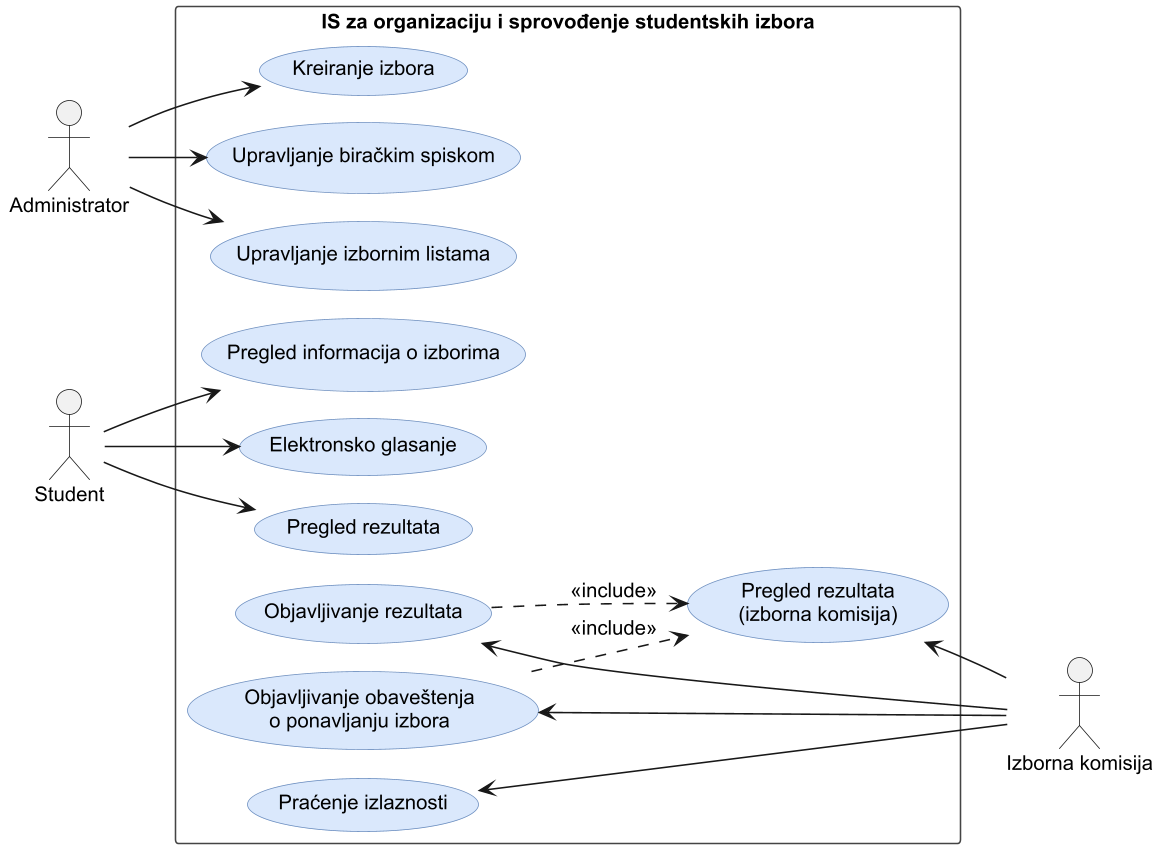
\includegraphics[width=\textwidth]{slucajevi_upotrebe.png}
    \caption{Dijagram slučajeva upotrebe}
    \label{fig:dijagram_slucajeva_upotrebe}
\end{figure}

U nastavku su detaljno opisani slučajevi upotrebe, grupisani po akterima, zajedno sa odgovarajućim dijagramima aktivnosti. Za ključne slučajeve upotrebe dati su i dijagrami sekvence. Slučajevi upotrebe 8, 9 i 10 čine jedan neprekidan tok rada izborne komisije, pa su opisani zajedno u okviru slučaja upotrebe \textit{Objavljivanje rezultata}.

\newpage
\subsection{Slučaj upotrebe: Kreiranje izbora}

\subsubsection*{Kratak opis}
Administrator kreira nove izbore i definiše period njihovog održavanja.

\subsubsection*{Akteri}
\begin{itemize}
    \item \textbf{Administrator} -- unosi podatke o izborima i potvrđuje njihovo kreiranje.
\end{itemize}

\subsubsection*{Preduslovi}
\begin{itemize}
    \item Administrator je prijavljen u sistem.
    \item Administrator ima ovlašćenje za kreiranje izbora.
\end{itemize}

\subsubsection*{Postuslovi}
\begin{itemize}
    \item U sistemu su evidentirani novi izbori sa definisanim periodom glasanja.
    \item Izbori još nisu spremni za glasanje, jer je potrebno formirati birački spisak i izborne liste.
\end{itemize}

\subsubsection*{Osnovni tok}
\begin{enumerate}
    \item Administrator bira opciju \textbf{Kreiraj izbore}.
    \item Sistem prikazuje formular za unos podataka o izborima.
    \item Administrator unosi naziv izbora, datum i vreme početka i datum i vreme kraja glasanja.
    \item Administrator potvrđuje unos.
    \item Sistem proverava ispravnost unetih podataka.
    \item Sistem čuva nove izbore i prikazuje poruku o uspešnom kreiranju.
\end{enumerate}

\subsubsection*{Alternativni tokovi}
\begin{enumerate}[label=\textbf{A\arabic*.}]
    \item \textbf{Neispravni ili nepotpuni podaci.} Ako administrator nije popunio sva polja ili je datum kraja glasanja pre datuma početka, sistem prikazuje poruku o grešci i omogućava ispravku podataka. Tok se nastavlja od koraka 3 osnovnog toka.
    \item \textbf{Odustajanje od kreiranja.} Administrator može da odustane od kreiranja izbora pre potvrde unosa. U tom slučaju sistem ne čuva podatke i slučaj upotrebe se završava.
\end{enumerate}

\begin{figure}[H]
    \centering
    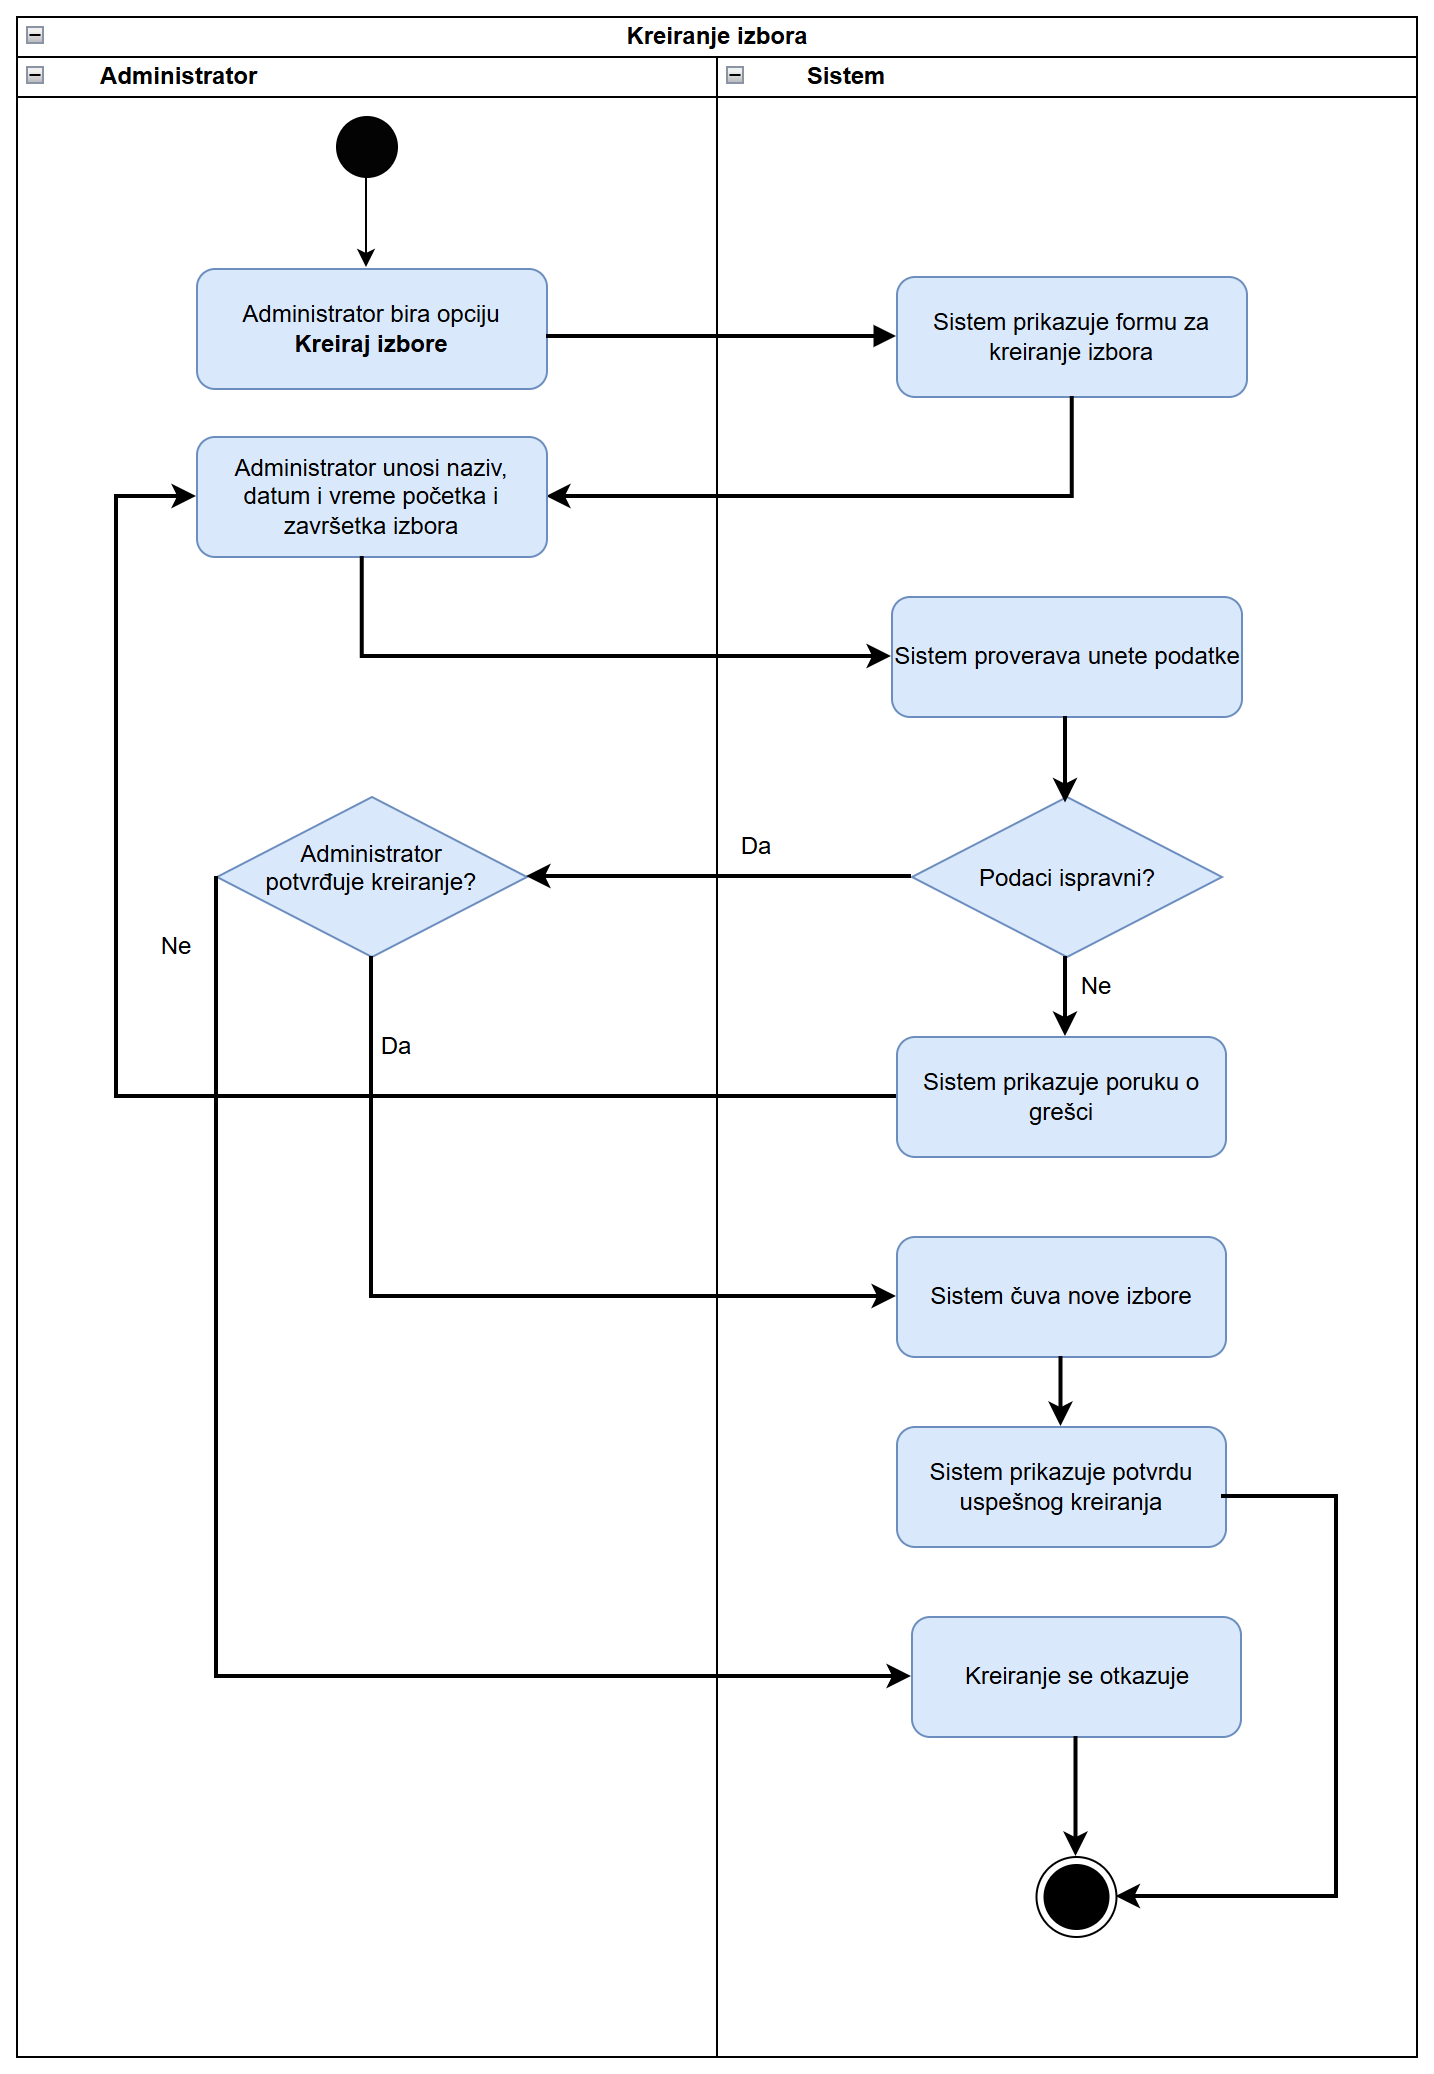
\includegraphics[width=0.8\textwidth]{kreiranje_izbora.png}
    \caption{Dijagram aktivnosti: Kreiranje izbora}
    \label{fig:kreiranje_izbora}
\end{figure}

\newpage

\subsection{Slučaj upotrebe: Upravljanje biračkim spiskom}

\subsubsection*{Kratak opis}
Administrator formira i ažurira birački spisak za izabrane izbore, odnosno spisak studenata koji imaju pravo glasa u skladu sa pravilima održavanja izbora.

\subsubsection*{Akteri}
\begin{itemize}
    \item \textbf{Administrator} -- učitava spisak studenata, dodaje ili uklanja pojedinačne studente i potvrđuje izmene.
\end{itemize}

\subsubsection*{Preduslovi}
\begin{itemize}
    \item Administrator je prijavljen u sistem.
    \item Izbori su kreirani u sistemu.
    \item Period glasanja za izabrane izbore još nije počeo.
\end{itemize}

\subsubsection*{Postuslovi}
\begin{itemize}
    \item Birački spisak za izabrane izbore je sačuvan u sistemu.
    \item Svaki student sa biračkog spiska ima status \textit{nije glasao}.
    \item Broj studenata sa pravom glasa je poznat i koristi se za računanje izlaznosti.
\end{itemize}

\subsubsection*{Osnovni tok}
\begin{enumerate}
    \item Administrator bira izbore i opciju \textbf{Birački spisak}.
    \item Sistem proverava da period glasanja još nije počeo.
    \item Sistem prikazuje trenutni birački spisak za izabrane izbore.
    \item Administrator učitava datoteku sa spiskom studenata ili ručno dodaje, odnosno uklanja pojedinačnog studenta.
    \item Sistem proverava format podataka, postojanje duplikata i da li svaki student ispunjava uslove za pravo glasa.
    \item Sistem prikazuje izmenjeni spisak i ukupan broj studenata sa pravom glasa.
    \item Administrator potvrđuje izmene.
    \item Sistem čuva birački spisak i prikazuje poruku o uspešnom čuvanju.
\end{enumerate}

\subsubsection*{Alternativni tokovi}
\begin{enumerate}[label=\textbf{A\arabic*.}]
    \item \textbf{Glasanje je već počelo.} Ako je u koraku 2 period glasanja već počeo, sistem prikazuje obaveštenje da birački spisak više ne može da se menja. Slučaj upotrebe se završava.
    \item \textbf{Neispravni podaci.} Ako u koraku 5 datoteka nije u očekivanom formatu, sadrži duplikate ili studente koji ne ispunjavaju uslove za pravo glasa, sistem prikazuje poruku o grešci sa spiskom problematičnih zapisa. Tok se nastavlja od koraka 4.
    \item \textbf{Odustajanje.} Ako administrator u koraku 7 ne potvrdi izmene, sistem ih odbacuje, a prethodno sačuvani birački spisak ostaje nepromenjen.
\end{enumerate}

\subsubsection*{Dodatne informacije}
Za svakog studenta na biračkom spisku čuvaju se ime i prezime, broj indeksa, studijski program i godina studija. Pravo glasa imaju studenti koji su upisani na fakultet u tekućoj školskoj godini.

\begin{figure}[H]
    \centering
    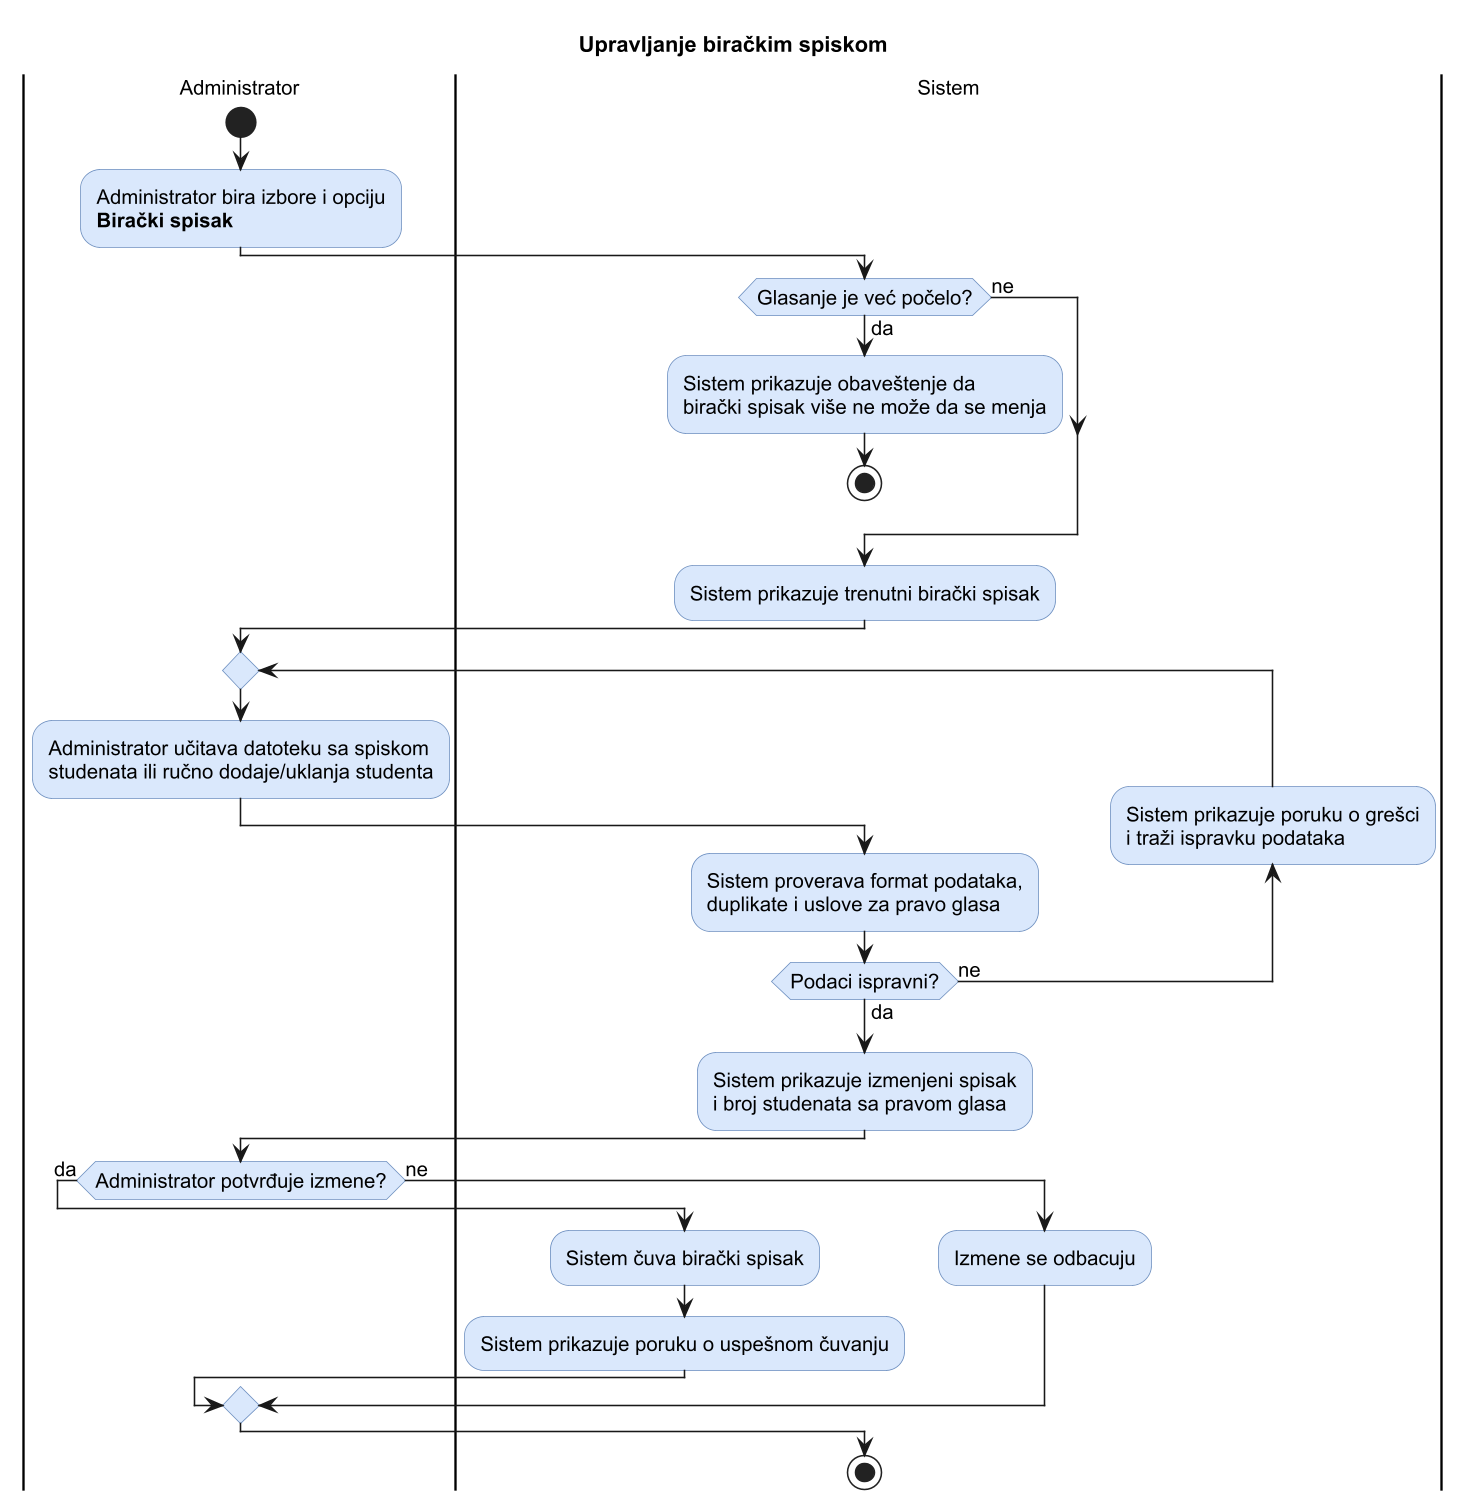
\includegraphics[width=0.85\textwidth]{aktivnosti_upravljanje_birackim_spiskom.png}
    \caption{Dijagram aktivnosti: Upravljanje biračkim spiskom}
    \label{fig:upravljanje_birackim_spiskom}
\end{figure}

\newpage

\subsection{Slučaj upotrebe: Upravljanje izbornim listama}

\subsubsection*{Kratak opis}
Administrator evidentira izborne liste koje učestvuju na izborima, kao i njihove izmene i uklanjanje pre početka glasanja.

\subsubsection*{Akteri}
\begin{itemize}
    \item \textbf{Administrator} -- dodaje, menja i uklanja izborne liste.
\end{itemize}

\subsubsection*{Preduslovi}
\begin{itemize}
    \item Administrator je prijavljen u sistem.
    \item Izbori su kreirani u sistemu.
    \item Period glasanja za izabrane izbore još nije počeo.
\end{itemize}

\subsubsection*{Postuslovi}
\begin{itemize}
    \item Izborne liste su evidentirane u sistemu i povezane sa izabranim izborima.
    \item Studenti mogu da pregledaju evidentirane izborne liste.
    \item Kada su formirani i birački spisak i izborne liste, izbori su spremni za glasanje.
\end{itemize}

\subsubsection*{Osnovni tok}
\begin{enumerate}
    \item Administrator bira izbore i opciju \textbf{Izborne liste}.
    \item Sistem proverava da period glasanja još nije počeo.
    \item Sistem prikazuje postojeće izborne liste za izabrane izbore.
    \item Administrator bira opciju \textbf{Dodaj listu}, \textbf{Izmeni listu} ili \textbf{Ukloni listu}.
    \item Administrator unosi naziv liste, nosioca liste i kratak opis programa.
    \item Sistem proverava da su sva obavezna polja popunjena i da je naziv liste jedinstven na izabranim izborima.
    \item Administrator potvrđuje izmenu.
    \item Sistem čuva izmene i prikazuje ažuriran spisak izbornih lista.
\end{enumerate}

\subsubsection*{Alternativni tokovi}
\begin{enumerate}[label=\textbf{A\arabic*.}]
    \item \textbf{Glasanje je već počelo.} Ako je u koraku 2 period glasanja već počeo, sistem prikazuje obaveštenje da izborne liste više ne mogu da se menjaju. Slučaj upotrebe se završava.
    \item \textbf{Neispravni podaci.} Ako u koraku 6 neko obavezno polje nije popunjeno ili lista sa istim nazivom već postoji, sistem prikazuje poruku o grešci. Tok se nastavlja od koraka 5.
    \item \textbf{Uklanjanje liste.} Ako administrator u koraku 4 izabere opciju \textbf{Ukloni listu}, korak 5 se preskače, a sistem pre koraka 7 traži potvrdu uklanjanja.
    \item \textbf{Odustajanje.} Ako administrator u koraku 7 ne potvrdi izmenu, sistem je odbacuje i izborne liste ostaju nepromenjene.
\end{enumerate}

\subsubsection*{Dodatne informacije}
Na izborima moraju da učestvuju najmanje dve izborne liste da bi izbori mogli da počnu.

\begin{figure}[H]
    \centering
    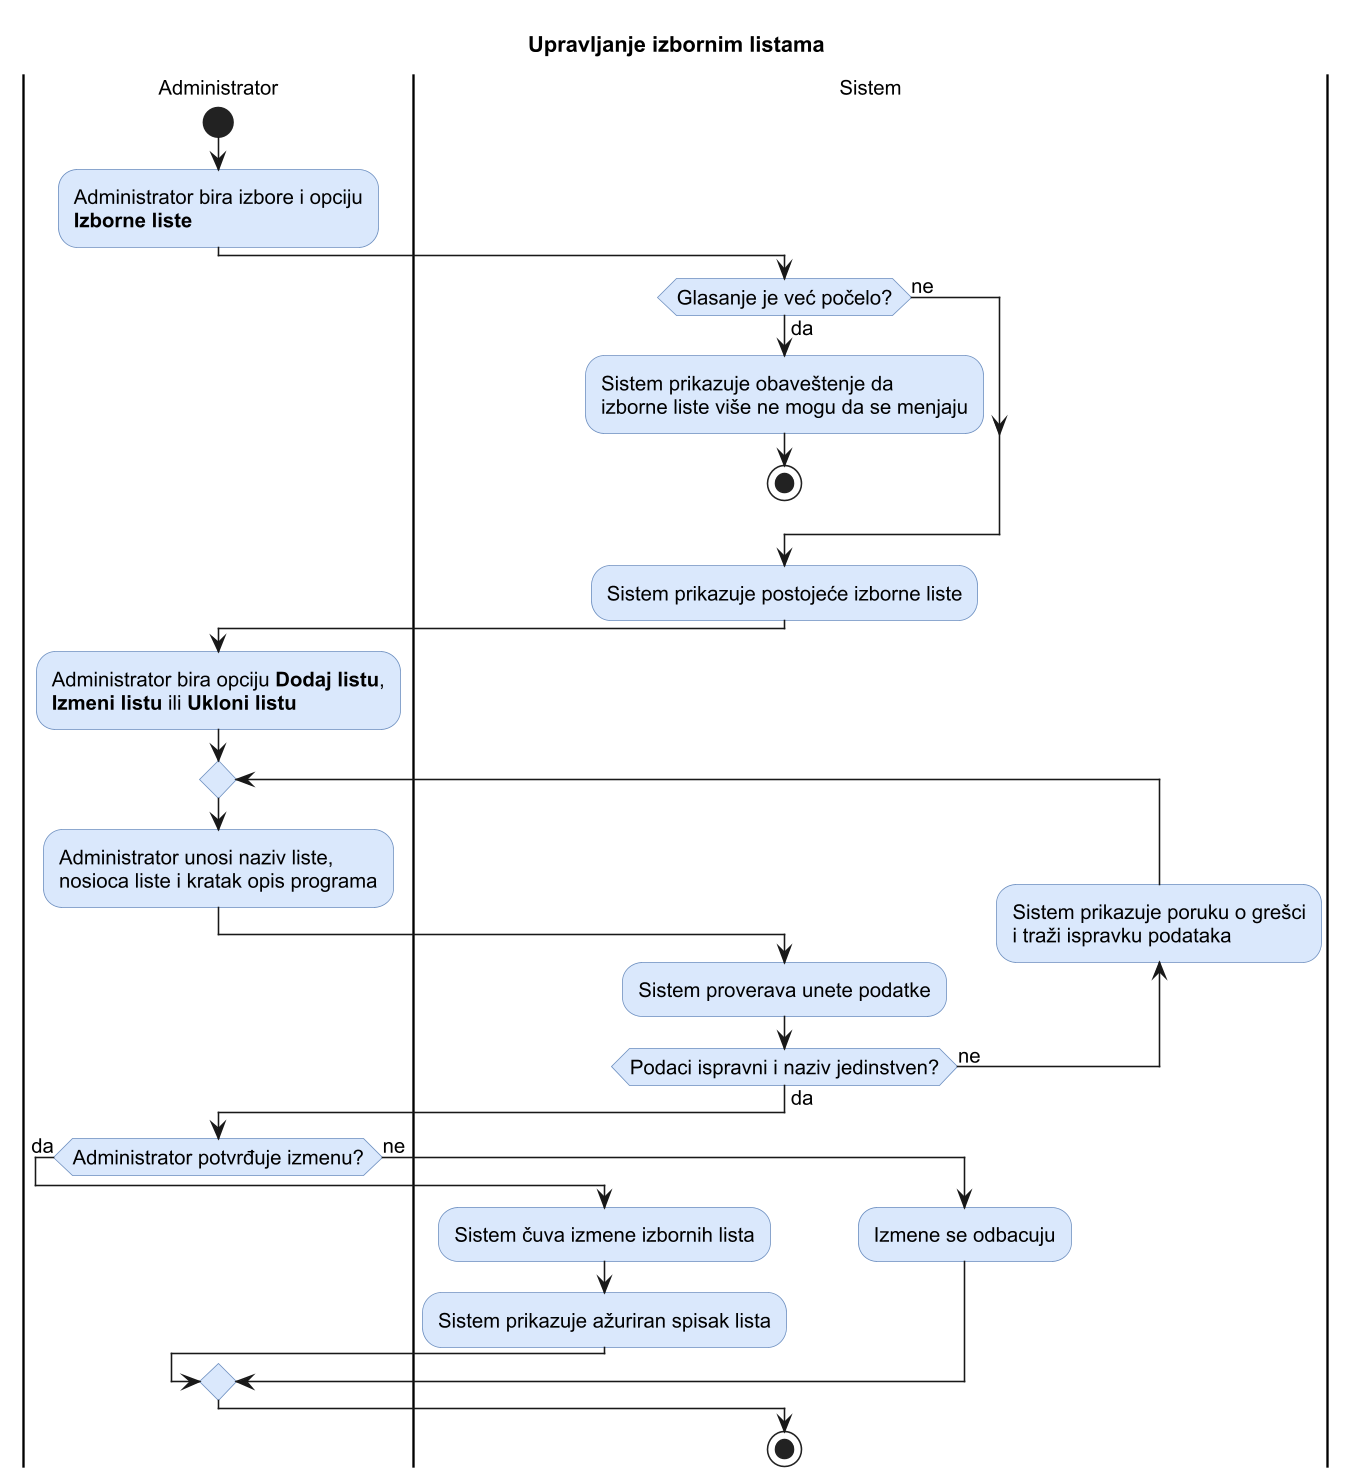
\includegraphics[width=0.85\textwidth]{aktivnosti_upravljanje_izbornim_listama.png}
    \caption{Dijagram aktivnosti: Upravljanje izbornim listama}
    \label{fig:upravljanje_izbornim_listama}
\end{figure}

\newpage

\subsection{Slučaj upotrebe: Pregled informacija o izborima}

\subsubsection*{Kratak opis}
Student pregleda raspisane izbore, period glasanja i izborne liste koje učestvuju na izborima, kao i informaciju o tome da li ima pravo glasa.

\subsubsection*{Akteri}
\begin{itemize}
    \item \textbf{Student} -- pregleda informacije o izborima i izbornim listama.
\end{itemize}

\subsubsection*{Preduslovi}
\begin{itemize}
    \item Student je prijavljen u sistem.
\end{itemize}

\subsubsection*{Postuslovi}
\begin{itemize}
    \item Student je upoznat sa periodom glasanja, izbornim listama i svojim pravom glasa.
    \item Stanje sistema se ne menja.
\end{itemize}

\subsubsection*{Osnovni tok}
\begin{enumerate}
    \item Student bira opciju \textbf{Izbori}.
    \item Sistem prikazuje spisak izbora sa periodom glasanja i statusom (\textit{najavljeni}, \textit{u toku}, \textit{završeni}).
    \item Student bira izbore.
    \item Sistem prikazuje detalje izbora i spisak izbornih lista sa nosiocima i opisom programa.
    \item Sistem prikazuje da li student ima pravo glasa na izabranim izborima i da li je već glasao.
    \item Student pregleda informacije o izbornim listama.
\end{enumerate}

\subsubsection*{Alternativni tokovi}
\begin{enumerate}[label=\textbf{A\arabic*.}]
    \item \textbf{Nema raspisanih izbora.} Ako u koraku 2 u sistemu ne postoje objavljeni izbori, sistem prikazuje poruku da trenutno nema raspisanih izbora. Slučaj upotrebe se završava.
    \item \textbf{Prelazak na glasanje.} Ako je glasanje u toku, a student ima pravo glasa i još nije glasao, student u koraku 6 može da izabere opciju \textbf{Glasaj}. Tada počinje slučaj upotrebe \textit{Elektronsko glasanje}.
\end{enumerate}

\begin{figure}[H]
    \centering
    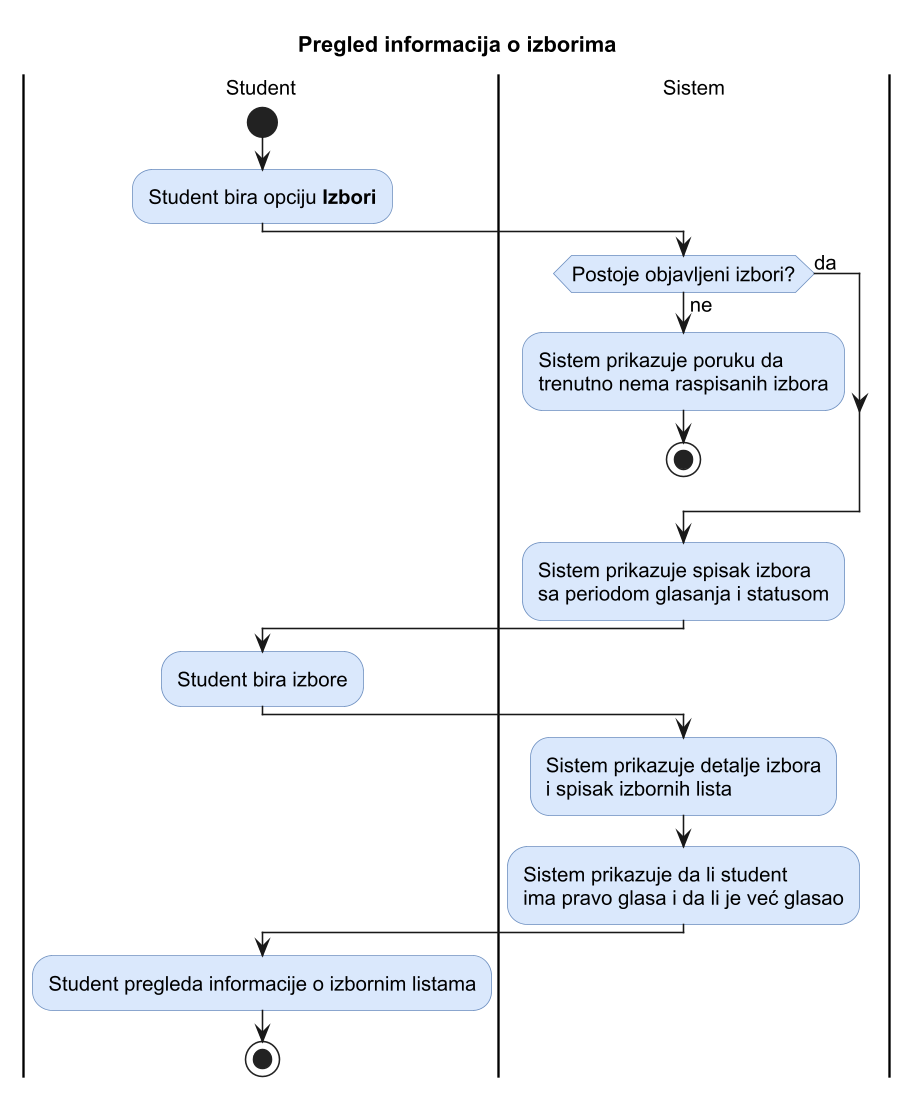
\includegraphics[width=0.7\textwidth]{aktivnosti_pregled_informacija.png}
    \caption{Dijagram aktivnosti: Pregled informacija o izborima}
    \label{fig:pregled_informacija}
\end{figure}

\newpage

\subsection{Slučaj upotrebe: Elektronsko glasanje}

\subsubsection*{Kratak opis}
Student koji ima pravo glasa, elektronski glasa za jednu od ponuđenih izbornih lista.

\subsubsection*{Akteri}
\begin{itemize}
    \item \textbf{Student} -- bira izbornu listu i potvrđuje svoj glas.
\end{itemize}

\subsubsection*{Preduslovi}
\begin{itemize}
    \item Student je prijavljen u sistem.
    \item Izbori su aktivni i period glasanja je u toku.
    \item Birački spisak i izborne liste su prethodno pripremljeni.
\end{itemize}

\subsubsection*{Postuslovi}
\begin{itemize}
    \item Glas je evidentiran bez povezivanja sa identitetom studenta.
    \item U sistemu je zabeleženo da je student glasao.
    \item Student ne može ponovo da glasa na istim izborima.
    \item Broj studenata koji su glasali je uvećan za jedan i ažuriran je procenat izlaznosti.
    \item Ako je student odustao od glasanja, ne menja se ni broj studenata koji su glasali ni procenat izlaznosti.
\end{itemize}

\subsubsection*{Osnovni tok}
\begin{enumerate}
    \item Student bira opciju \textbf{Glasaj}.
    \item Sistem proverava da li student ima pravo glasa i da li je već glasao.
    \item Ako student ima pravo glasa i još nije glasao, sistem prikazuje dostupne izborne liste.
    \item Student bira jednu izbornu listu.
    \item Sistem prikazuje izabranu listu i traži potvrdu glasanja.
    \item Student potvrđuje izbor.
    \item Sistem anonimno evidentira glas i beleži da je student iskoristio pravo glasa.
    \item Sistem prikazuje poruku da je glas uspešno evidentiran.
\end{enumerate}

\subsubsection*{Alternativni tokovi}
\begin{enumerate}[label=\textbf{A\arabic*.}]
    \item \textbf{Student nema pravo glasa.} Ako se student ne nalazi na biračkom spisku, sistem u koraku 2 prikazuje obaveštenje da student nema pravo glasa i ne dozvoljava nastavak. Slučaj upotrebe se završava.
    \item \textbf{Student je već glasao.} Ako je student već glasao na ovim izborima, sistem u koraku 2 prikazuje odgovarajuće obaveštenje i ne dozvoljava ponovno glasanje. Slučaj upotrebe se završava.
    \item \textbf{Student odustaje od glasanja.} Ako student u koraku 6 ne potvrdi izbor, glas se ne evidentira i student može da napusti postupak. Status studenta ostaje \textit{nije glasao} i on može ponovo da pristupi glasanju dok ono traje.
\end{enumerate}

\begin{figure}[H]
    \centering
    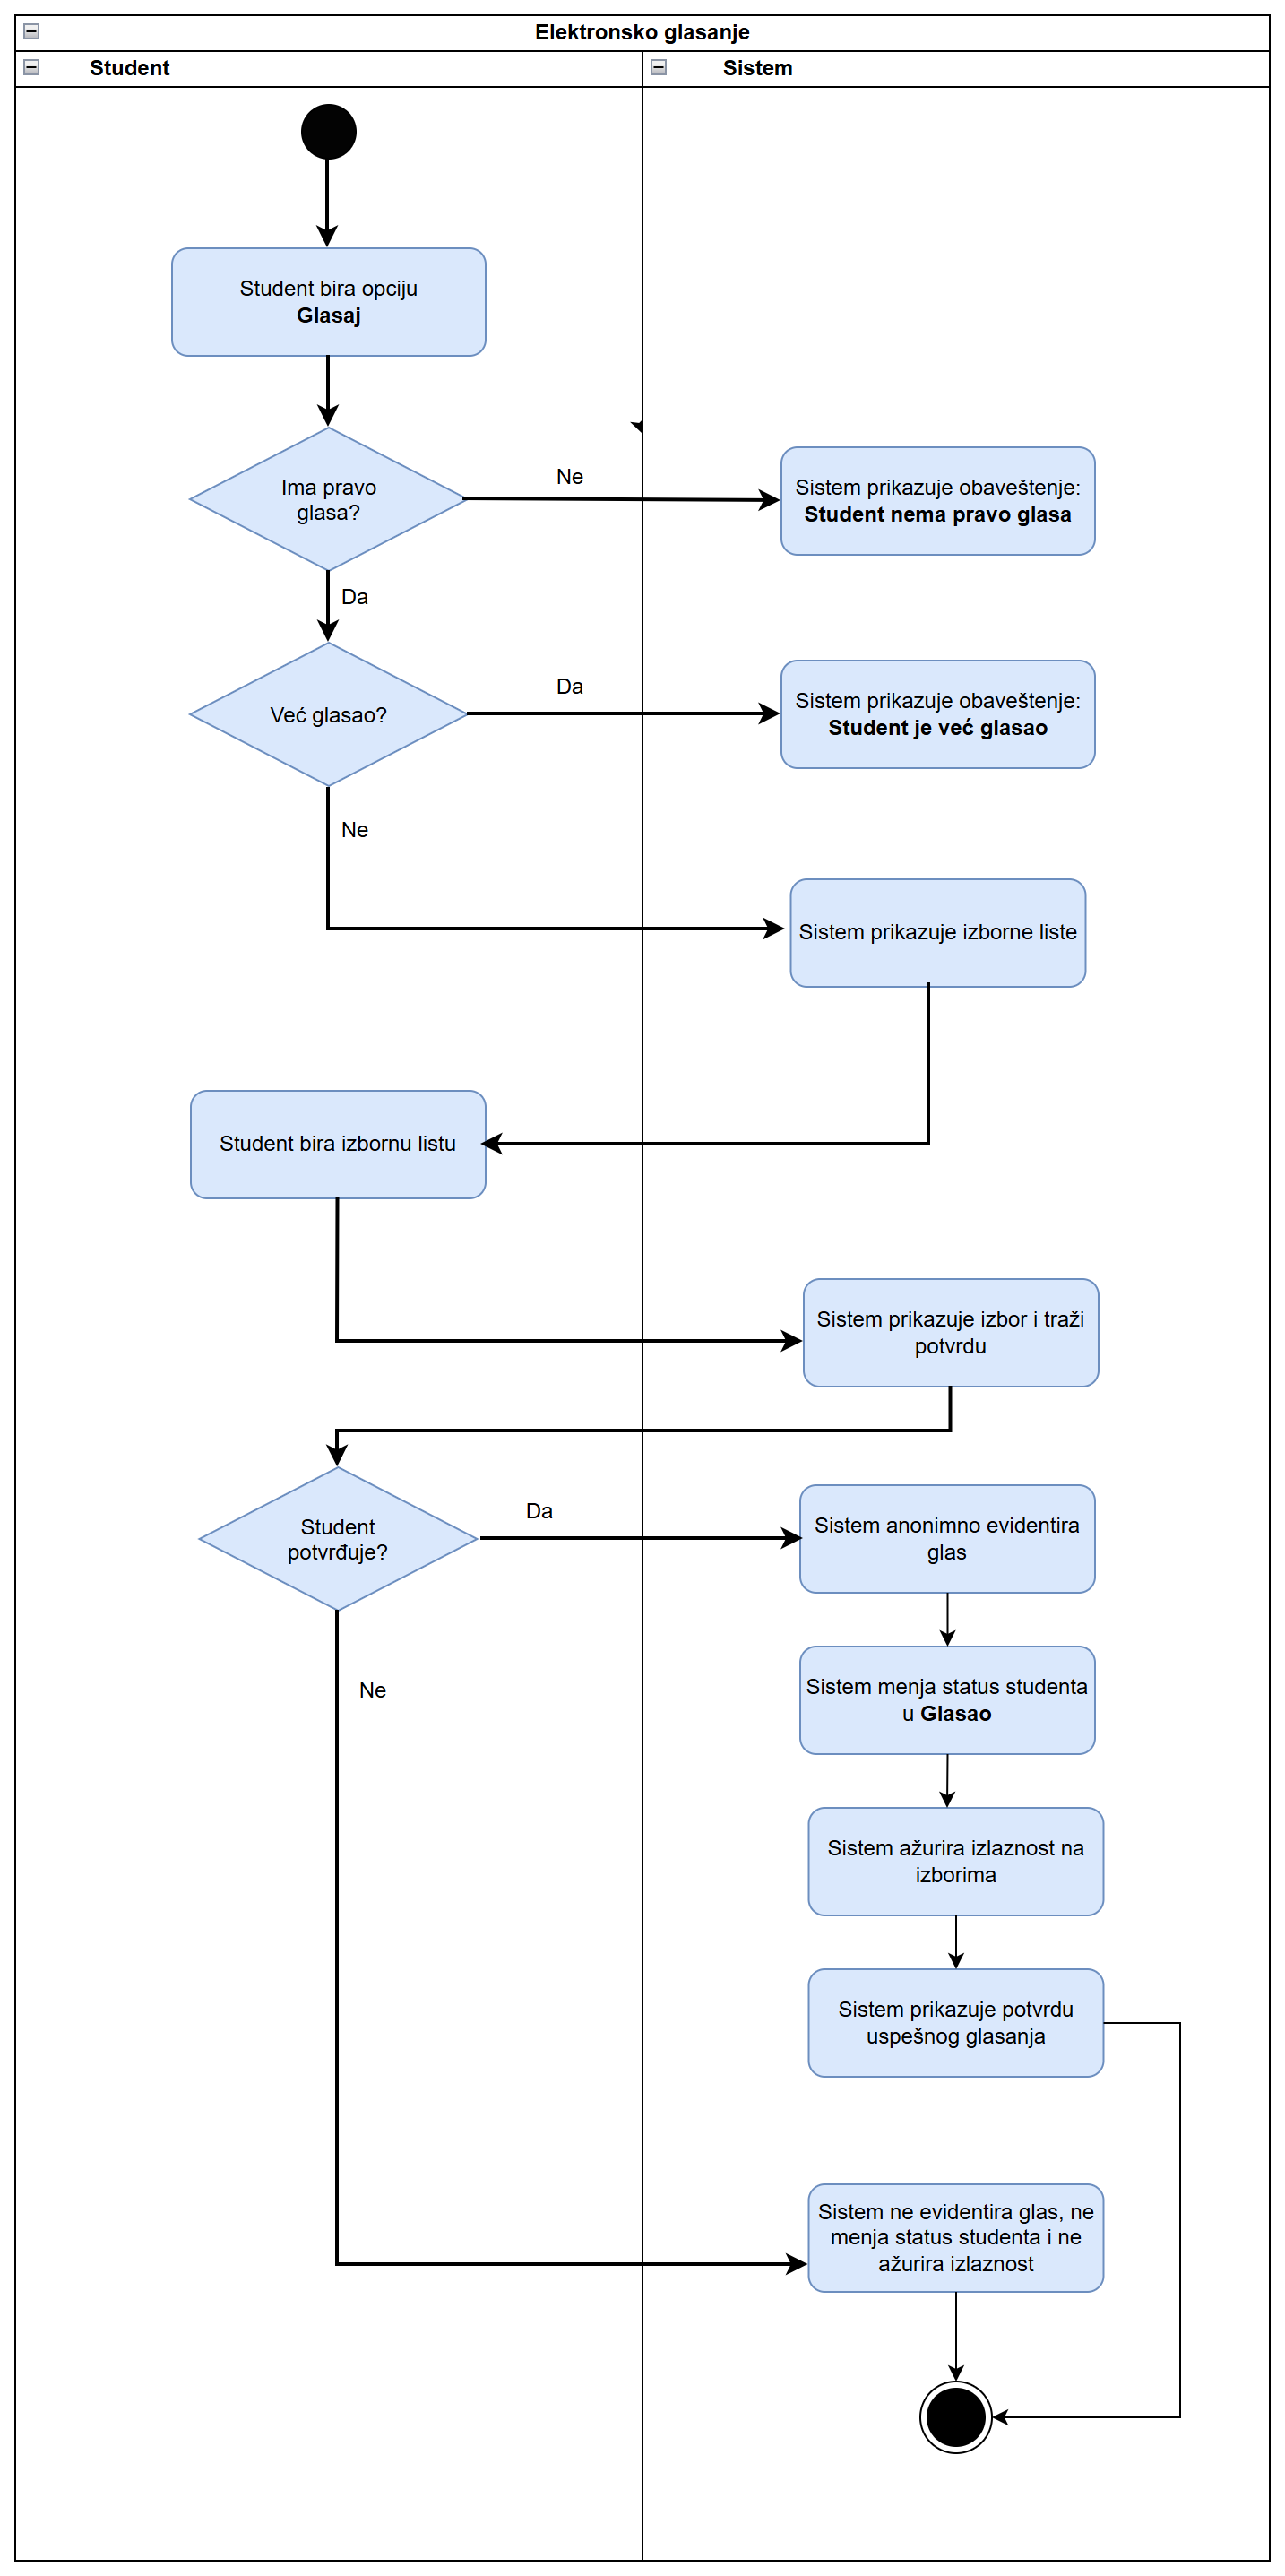
\includegraphics[height=0.8\textheight]{elektronsko_glasanje.png}
    \caption{Dijagram aktivnosti: Elektronsko glasanje}
    \label{fig:elektronsko_glasanje}
\end{figure}

\begin{figure}[H]
    \centering
    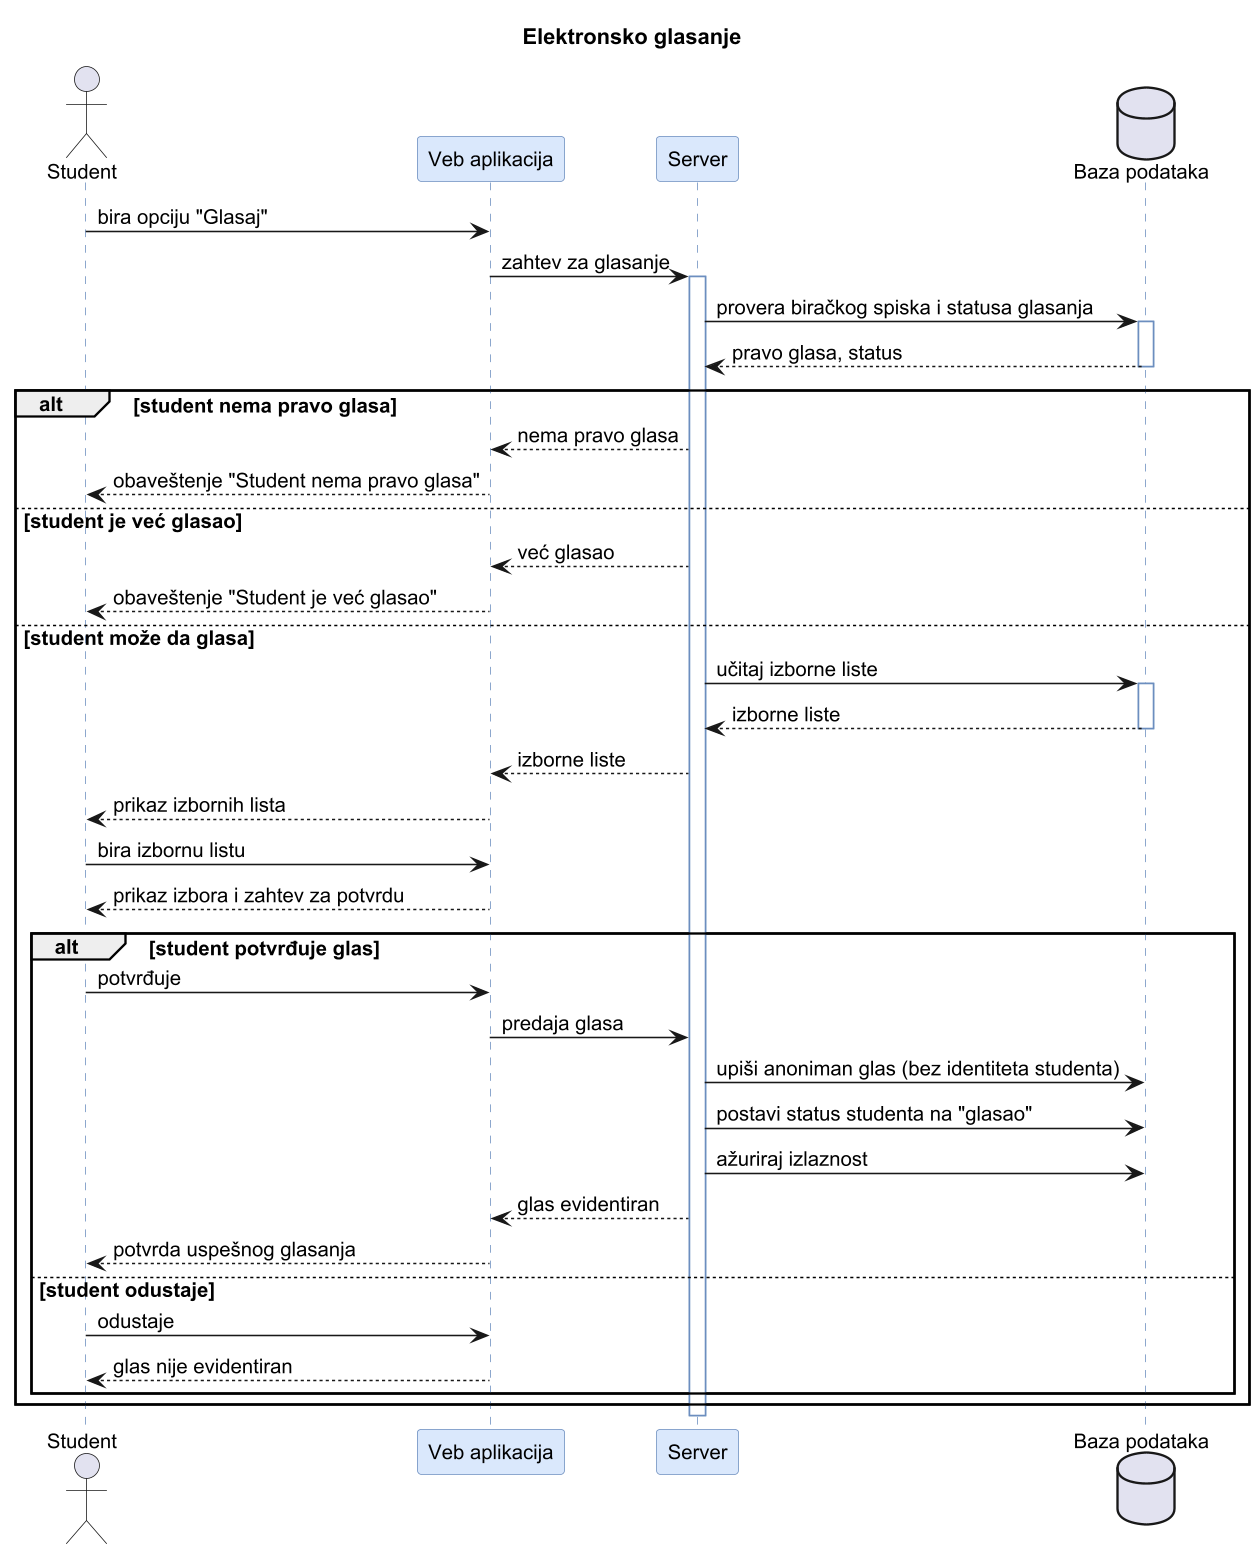
\includegraphics[width=\textwidth,height=0.8\textheight,keepaspectratio]{sekvenca_elektronsko_glasanje.png}
    \caption{Dijagram sekvence: Elektronsko glasanje}
    \label{fig:sekvenca_elektronsko_glasanje}
\end{figure}

\newpage

\subsection{Slučaj upotrebe: Pregled rezultata}

\subsubsection*{Kratak opis}
Student pregleda objavljene rezultate završenih izbora ili, ukoliko izbori nisu uspeli, obaveštenje o ponavljanju izbora.

\subsubsection*{Akteri}
\begin{itemize}
    \item \textbf{Student} -- pregleda rezultate izbora.
\end{itemize}

\subsubsection*{Preduslovi}
\begin{itemize}
    \item Student je prijavljen u sistem.
    \item Period glasanja za izabrane izbore je završen.
\end{itemize}

\subsubsection*{Postuslovi}
\begin{itemize}
    \item Student je upoznat sa ishodom izbora.
    \item Stanje sistema se ne menja.
\end{itemize}

\subsubsection*{Osnovni tok}
\begin{enumerate}
    \item Student bira završene izbore i opciju \textbf{Rezultati}.
    \item Sistem proverava status izbora.
    \item Ako je izborna komisija objavila rezultate, sistem prikazuje procenat izlaznosti i broj glasova koji je dobila svaka izborna lista.
    \item Student pregleda rezultate.
\end{enumerate}

\subsubsection*{Alternativni tokovi}
\begin{enumerate}[label=\textbf{A\arabic*.}]
    \item \textbf{Izbori se ponavljaju.} Ako je u koraku 2 izborna komisija objavila obaveštenje o ponavljanju izbora, sistem prikazuje obaveštenje da izbori nisu važeći zbog nedovoljne izlaznosti i da će biti ponovljeni.
    \item \textbf{Rezultati još nisu objavljeni.} Ako u koraku 2 izborna komisija još nije objavila ni rezultate ni obaveštenje, sistem prikazuje poruku da rezultati još nisu objavljeni.
\end{enumerate}

\begin{figure}[H]
    \centering
    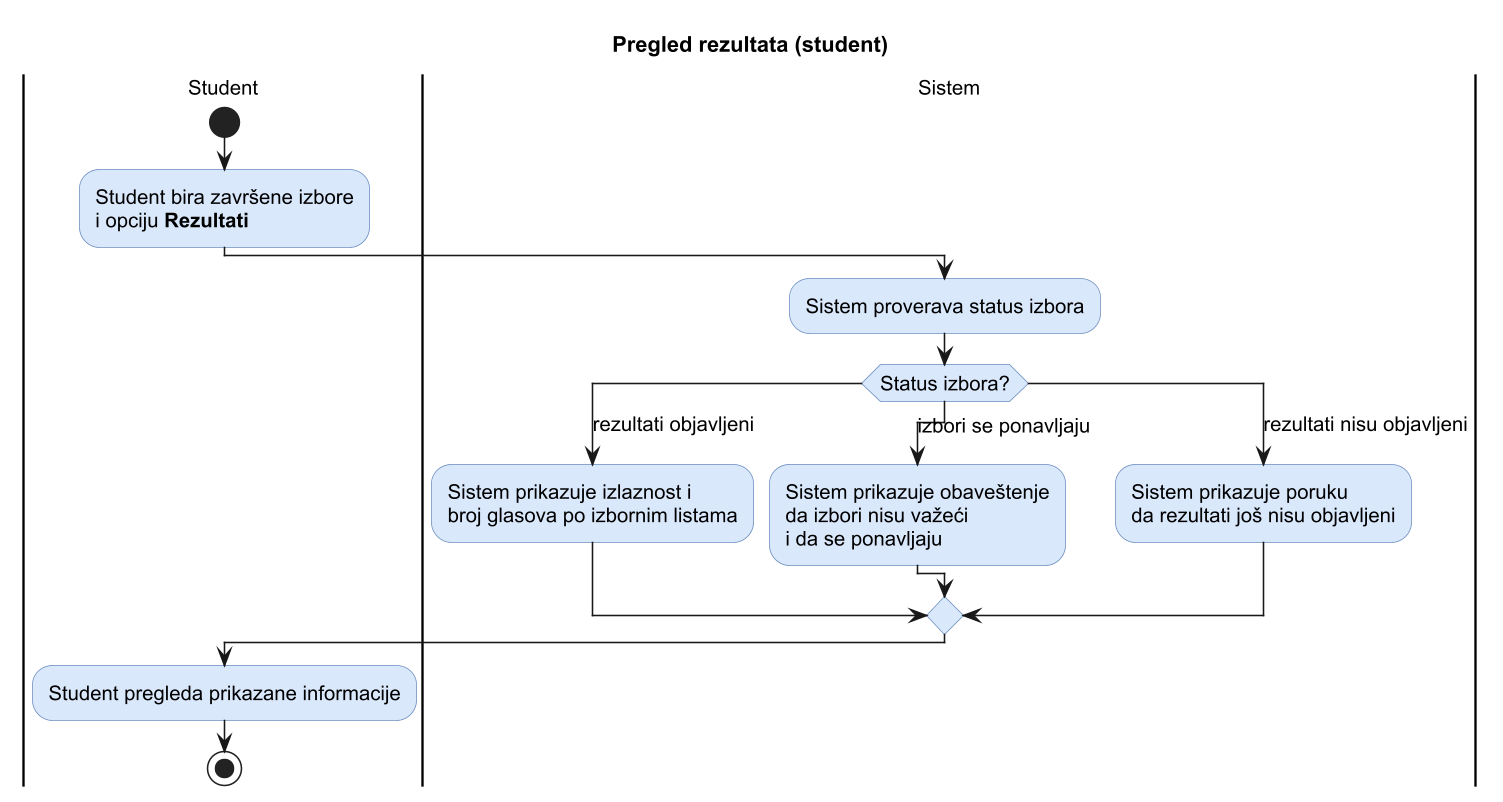
\includegraphics[width=\textwidth]{aktivnosti_pregled_rezultata.png}
    \caption{Dijagram aktivnosti: Pregled rezultata}
    \label{fig:pregled_rezultata}
\end{figure}

\newpage

\subsection{Slučaj upotrebe: Praćenje izlaznosti}

\subsubsection*{Kratak opis}
Član izborne komisije tokom trajanja glasanja prati broj studenata sa pravom glasa, broj studenata koji su glasali i procenat izlaznosti.

\subsubsection*{Akteri}
\begin{itemize}
    \item \textbf{Član izborne komisije} -- prati izlaznost tokom glasanja.
\end{itemize}

\subsubsection*{Preduslovi}
\begin{itemize}
    \item Član izborne komisije je prijavljen u sistem.
    \item Period glasanja za izabrane izbore je počeo.
\end{itemize}

\subsubsection*{Postuslovi}
\begin{itemize}
    \item Član komisije ima uvid u trenutnu izlaznost.
    \item Stanje sistema se ne menja.
\end{itemize}

\subsubsection*{Osnovni tok}
\begin{enumerate}
    \item Član komisije bira izbore i opciju \textbf{Praćenje izlaznosti}.
    \item Sistem proverava da je period glasanja počeo.
    \item Sistem računa broj studenata sa pravom glasa, broj studenata koji su glasali i procenat izlaznosti.
    \item Sistem prikazuje trenutnu izlaznost.
    \item Član komisije prati izlaznost i, po potrebi, osvežava prikaz. Tok se tada nastavlja od koraka 3.
\end{enumerate}

\subsubsection*{Alternativni tokovi}
\begin{enumerate}[label=\textbf{A\arabic*.}]
    \item \textbf{Glasanje još nije počelo.} Ako u koraku 2 period glasanja još nije počeo, sistem prikazuje poruku da glasanje još nije počelo. Slučaj upotrebe se završava.
\end{enumerate}

\subsubsection*{Dodatne informacije}
Sistem prikazuje samo zbirne podatke o izlaznosti. Tokom glasanja nije dostupan uvid u to za koju su listu studenti glasali niti koji su studenti glasali, čime se čuva tajnost glasanja.

\begin{figure}[H]
    \centering
    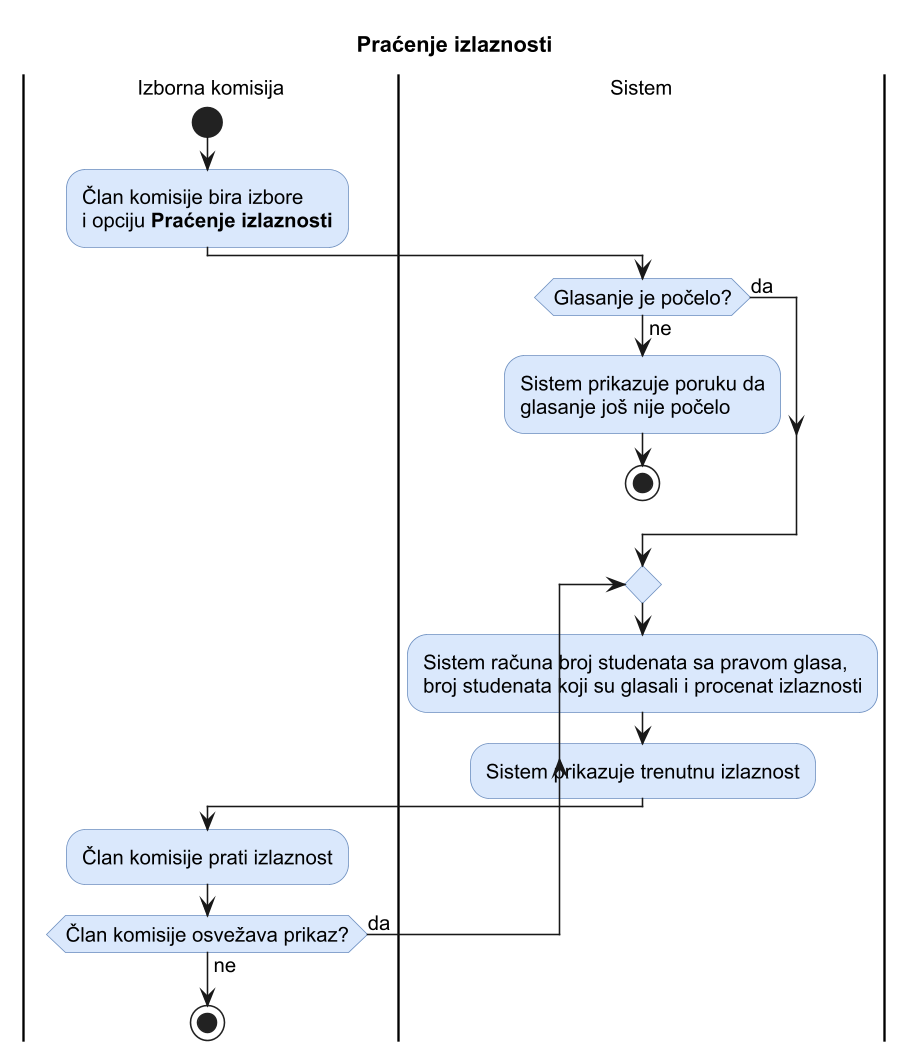
\includegraphics[width=0.7\textwidth]{aktivnosti_pracenje_izlaznosti.png}
    \caption{Dijagram aktivnosti: Praćenje izlaznosti}
    \label{fig:pracenje_izlaznosti}
\end{figure}

\newpage

\subsection{Slučaj upotrebe: Objavljivanje rezultata}

\subsubsection*{Kratak opis}
Izborna komisija objavljuje rezultate završenih izbora ili, ukoliko nije ispunjen uslov minimalne izlaznosti, obaveštenje o potrebi ponavljanja izbora.

\subsubsection*{Akteri}
\begin{itemize}
    \item \textbf{Član izborne komisije} -- pregleda izlaznost i rezultate i potvrđuje njihovo objavljivanje.
\end{itemize}

\subsubsection*{Preduslovi}
\begin{itemize}
    \item Član izborne komisije je prijavljen u sistem.
    \item Period glasanja je završen.
    \item Sistem je evidentirao i prebrojao glasove.
\end{itemize}

\subsubsection*{Postuslovi}
\begin{itemize}
    \item Ako je izlaznost veća ili jednaka 50\% i komisija potvrdi objavljivanje, rezultati postaju dostupni studentima.
    \item Ako je izlaznost manja od 50\% i komisija potvrdi objavljivanje obaveštenja, studenti dobijaju informaciju da se izbori ponavljaju.
    \item Ako komisija odustane od objavljivanja, status izbora ostaje nepromenjen.
\end{itemize}

\subsubsection*{Osnovni tok}
\begin{enumerate}
    \item Član komisije bira opciju \textbf{Pregled rezultata}.
    \item Sistem prikazuje broj studenata sa pravom glasa, broj studenata koji su glasali i procenat izlaznosti.
    \item Sistem proverava da li je izlaznost veća ili jednaka 50\%.
    \item Ako je uslov ispunjen, sistem prikazuje rezultate glasanja, odnosno broj glasova koji je dobila svaka izborna lista.
    \item Član komisije pregleda rezultate.
    \item Član komisije bira opciju \textbf{Objavi}.
    \item Sistem objavljuje rezultate i prikazuje poruku o uspešnom objavljivanju.
\end{enumerate}

\subsubsection*{Alternativni tokovi}
\begin{enumerate}[label=\textbf{A\arabic*.}]
    \item \textbf{Izlaznost je manja od 50\%.} Sistem u koraku 3 prikazuje obaveštenje da izbori nisu važeći. Član komisije bira opciju za objavljivanje obaveštenja o ponavljanju izbora. Sistem objavljuje obaveštenje koje je dostupno studentima, a rezultati se ne objavljuju kao važeći. Slučaj upotrebe se završava.
    \item \textbf{Odustajanje od objavljivanja.} Ako član komisije ne potvrdi objavljivanje, sistem ne objavljuje ni rezultate ni obaveštenje. Komisija kasnije može ponovo da pristupi ovoj funkcionalnosti.
\end{enumerate}

\begin{figure}[H]
    \centering
    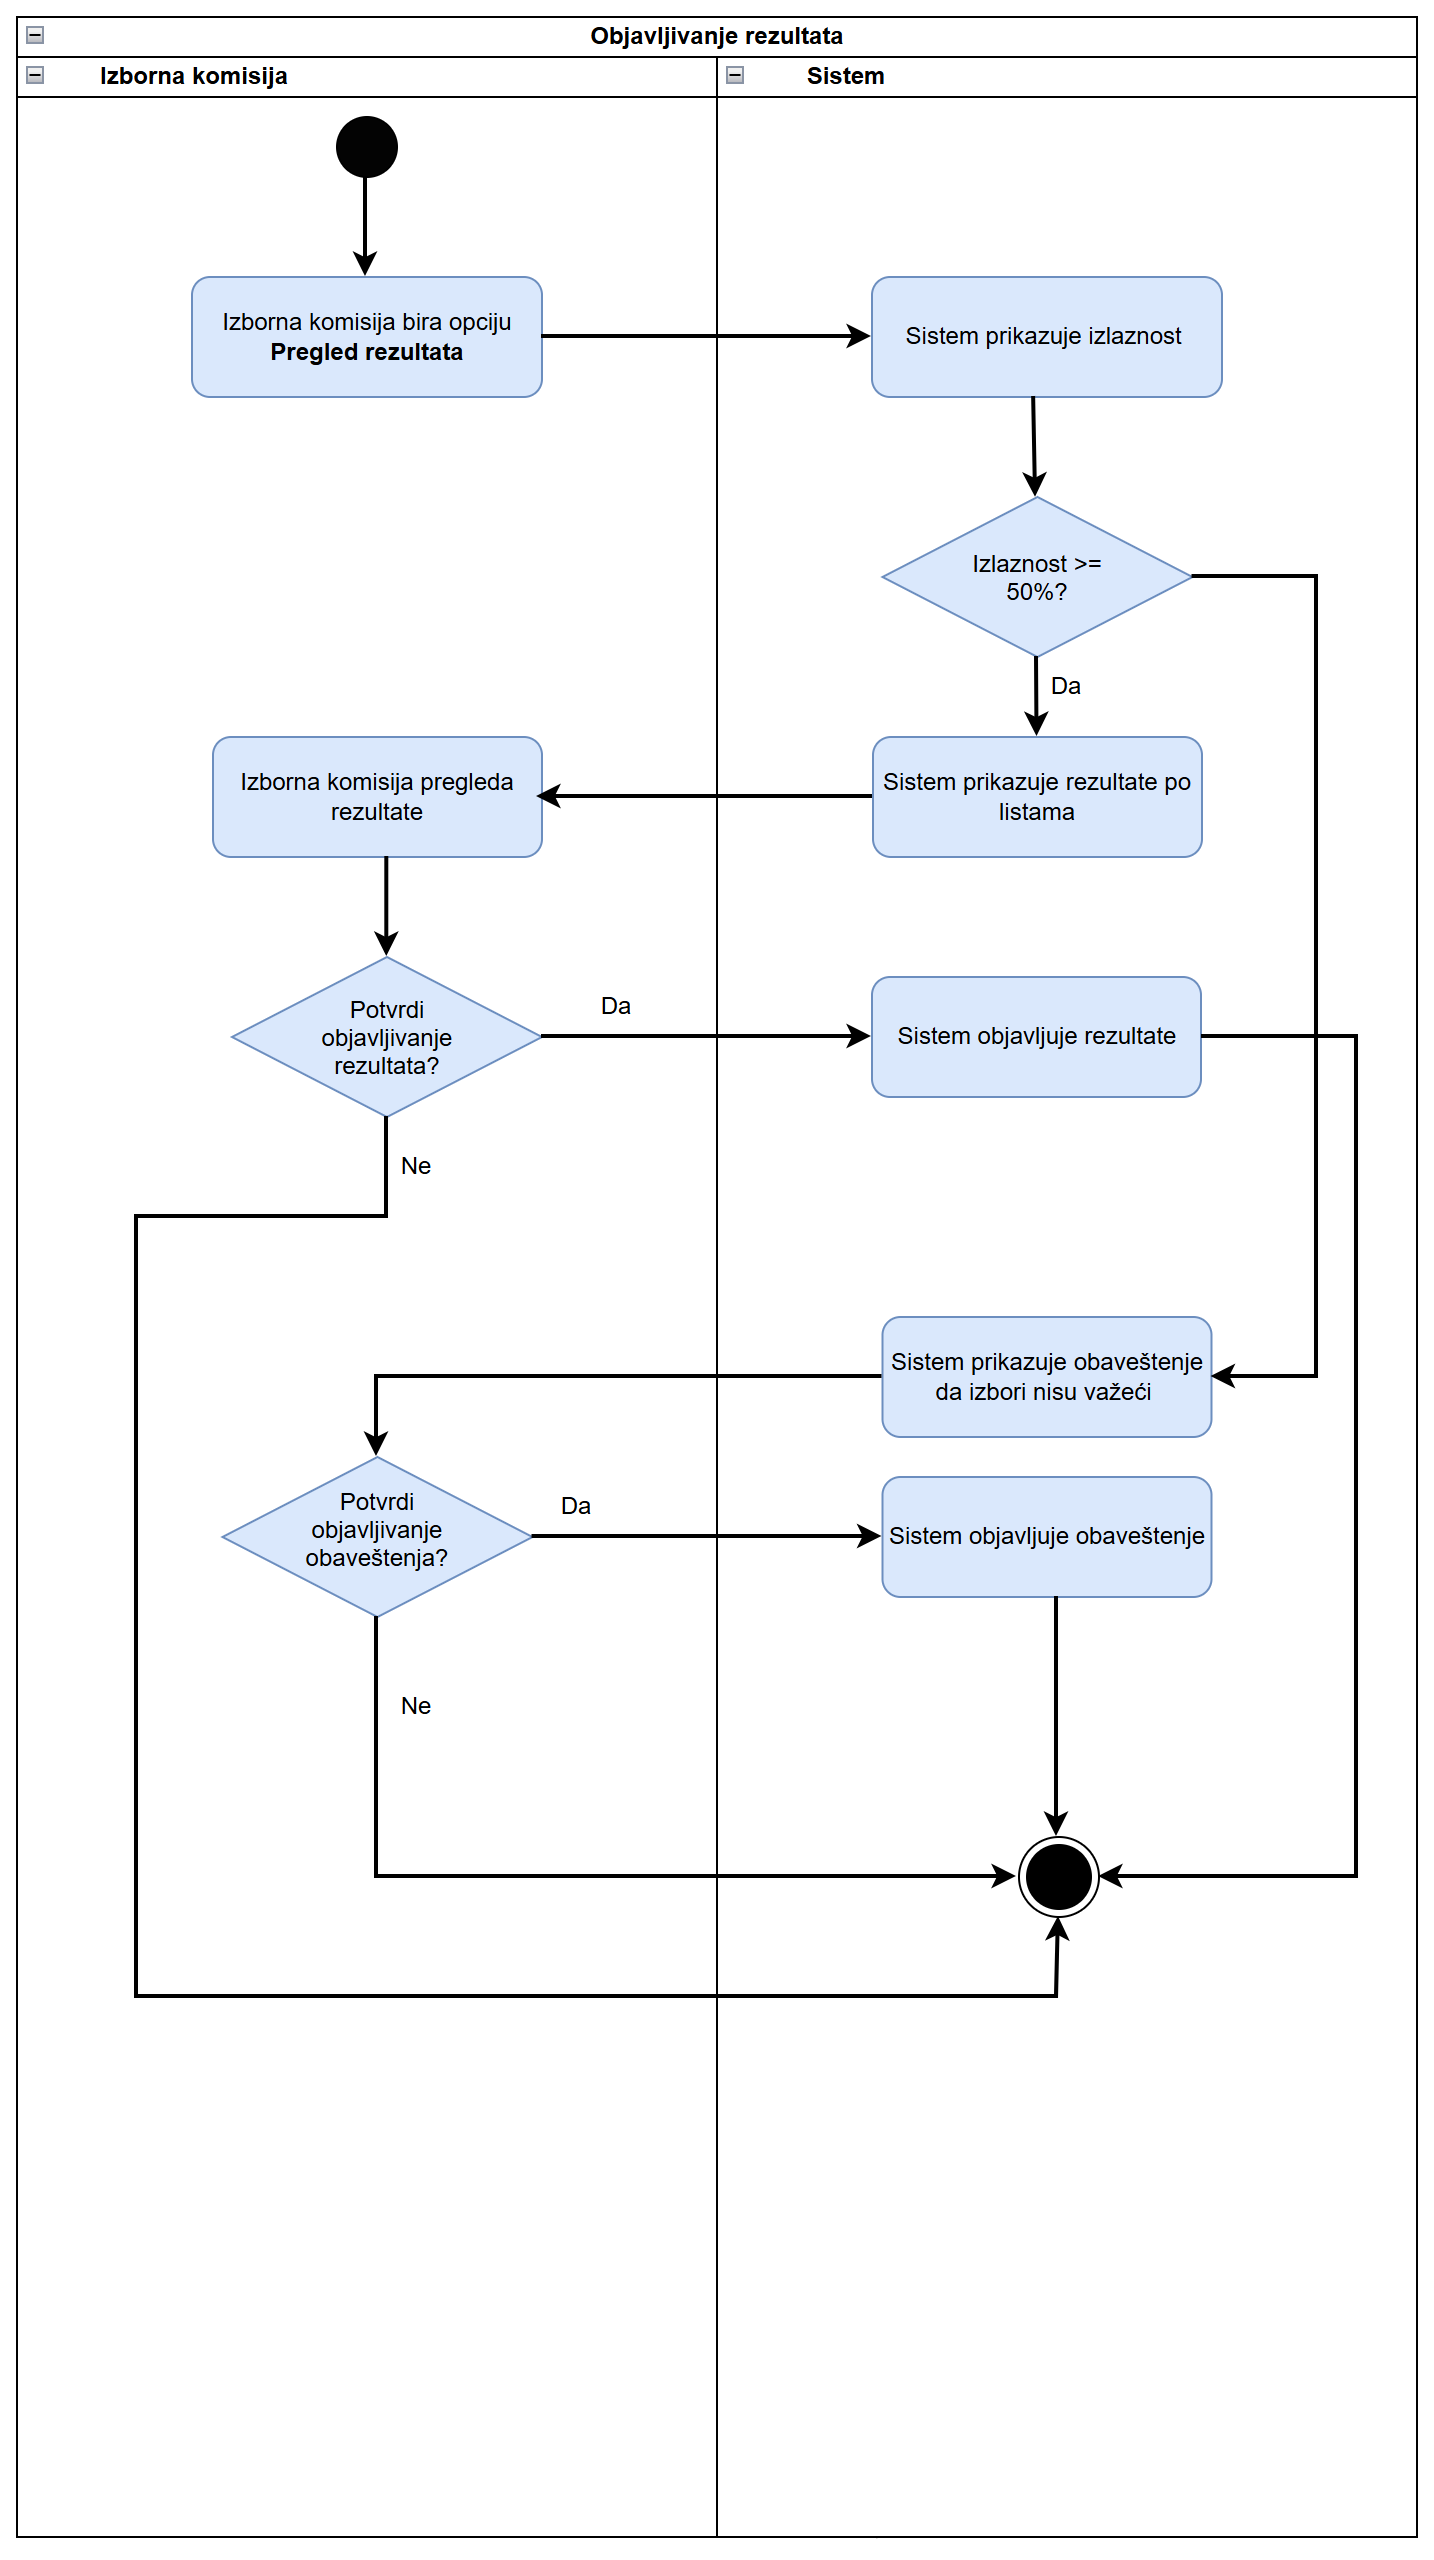
\includegraphics[height=0.8\textheight]{objavljivanje_rezultata.png}
    \caption{Dijagram aktivnosti: Objavljivanje rezultata}
    \label{fig:objavljivanje_rezultata}
\end{figure}

\begin{figure}[H]
    \centering
    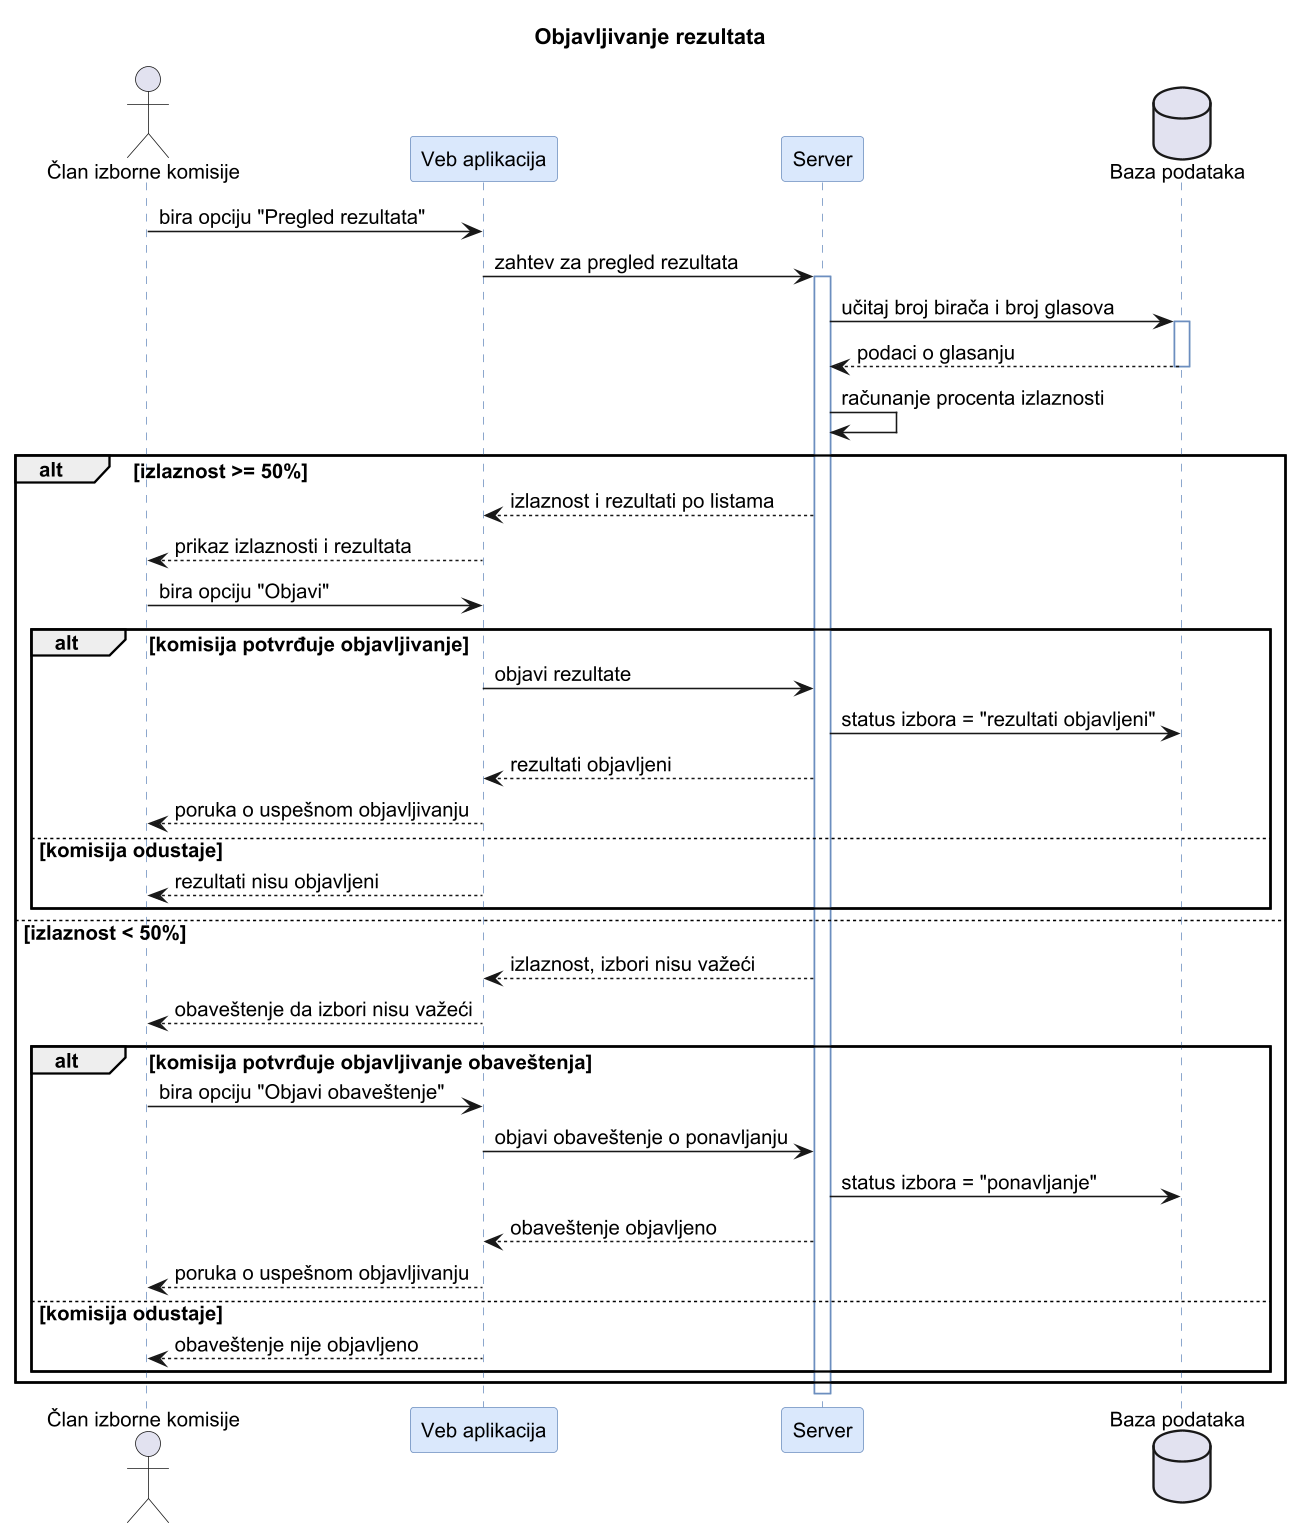
\includegraphics[width=\textwidth,height=0.8\textheight,keepaspectratio]{sekvenca_objavljivanje_rezultata.png}
    \caption{Dijagram sekvence: Objavljivanje rezultata}
    \label{fig:sekvenca_objavljivanje_rezultata}
\end{figure}

\newpage


% ====================== DIJAGRAMI TOKA PODATAKA ==================
\section{Dijagrami toka podataka}
Dijagrami toka podataka (DFD) prikazuju kako podaci ulaze u sistem, kako ih procesi obrađuju i gde se čuvaju. Najpre je dat dijagram konteksta, koji sistem prikazuje kao jedan proces u interakciji sa spoljnim entitetima, a zatim dijagram prvog nivoa, na kome je sistem razložen na osnovne procese i skladišta podataka.

\subsection{Dijagram konteksta}

Spoljni entiteti sistema su administrator, student i izborna komisija. Administrator unosi podatke o izborima, birački spisak i izborne liste, a od sistema dobija potvrde i poruke o greškama. Student šalje zahtev za glasanje i izabranu listu, a dobija informacije o izborima, potvrdu glasanja i rezultate, odnosno obaveštenje o ponavljanju izbora. Izborna komisija od sistema dobija podatke o izlaznosti i rezultate glasanja, a sistemu šalje potvrdu objavljivanja.

\begin{figure}[H]
    \centering
    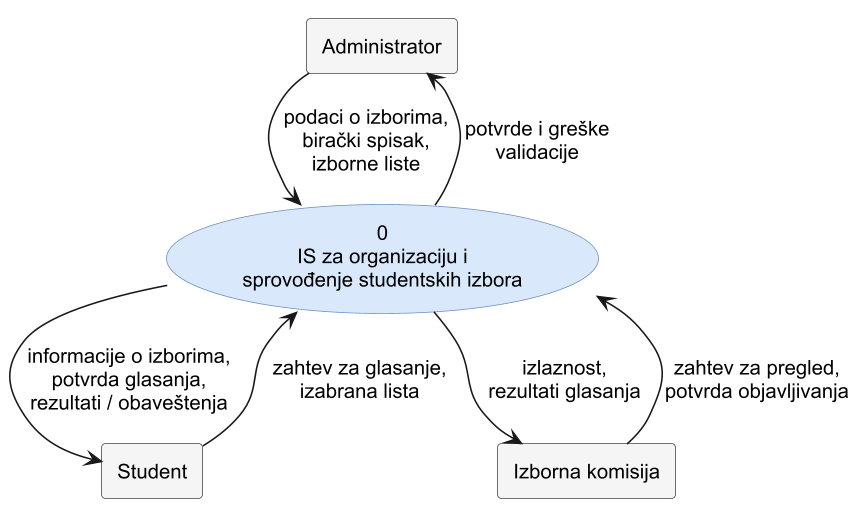
\includegraphics[width=0.85\textwidth]{dfd_kontekst.png}
    \caption{DFD -- dijagram konteksta}
    \label{fig:dfd_kontekst}
\end{figure}

\subsection{Dijagram prvog nivoa}

Na dijagramu prvog nivoa sistem je razložen na šest procesa:
\begin{enumerate}
    \item \textbf{Upravljanje izborima} -- čuva nove izbore sa periodom glasanja u skladištu \textit{D1 Izbori}.
    \item \textbf{Upravljanje biračkim spiskom} -- formira spisak studenata sa pravom glasa u skladištu \textit{D2 Birački spisak}.
    \item \textbf{Upravljanje izbornim listama} -- čuva izborne liste u skladištu \textit{D3 Izborne liste}.
    \item \textbf{Glasanje} -- proverava pravo glasa, upisuje anoniman glas u skladište \textit{D4 Glasovi} i beleži da je student glasao. Glas i identitet studenta se čuvaju u odvojenim skladištima, čime se obezbeđuje tajnost glasanja.
    \item \textbf{Praćenje izlaznosti} -- na osnovu biračkog spiska računa izlaznost i prikazuje je izbornoj komisiji.
    \item \textbf{Obrada i objavljivanje rezultata} -- prebrojava glasove, proverava uslov izlaznosti i, nakon potvrde komisije, objavljuje rezultate ili obaveštenje o ponavljanju izbora.
\end{enumerate}

\begin{figure}[H]
    \centering
    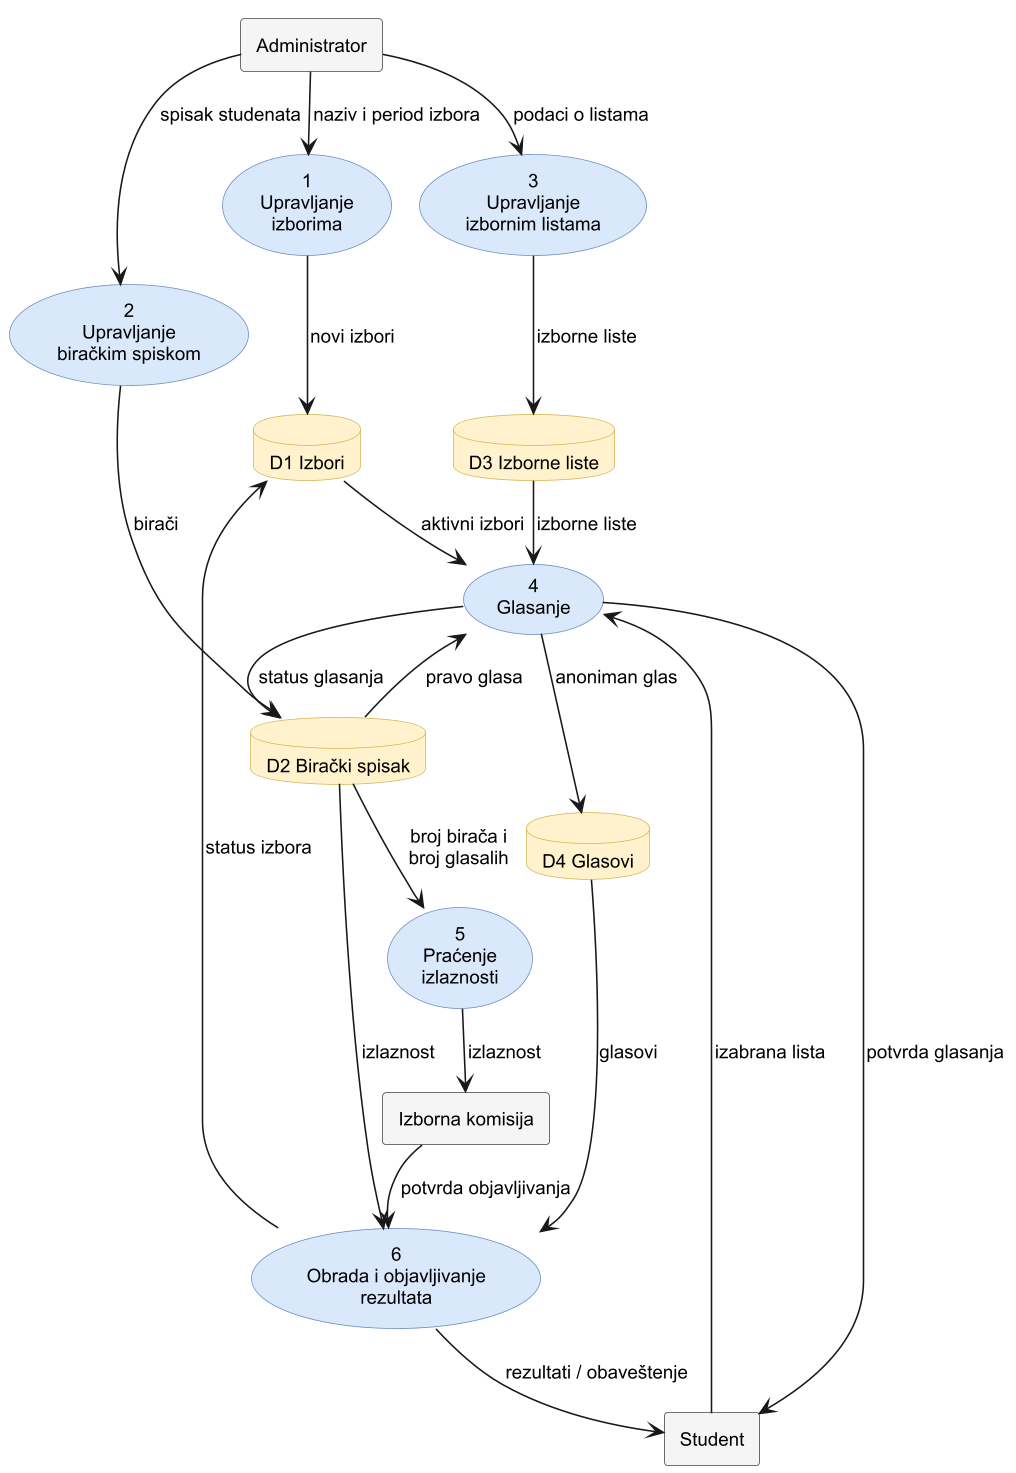
\includegraphics[height=0.72\textheight]{dfd_nivo1.png}
    \caption{DFD -- dijagram prvog nivoa}
    \label{fig:dfd_nivo1}
\end{figure}

\newpage


% ========================= POSLOVNI PROCESI =======================
\section{BPMN dijagrami}
BPMN dijagrami prikazuju celokupan poslovni proces sprovođenja studentskih izbora i ulogu svakog učesnika u njemu. Proces je podeljen na dva dela: pripremu i sprovođenje glasanja i obradu i objavljivanje rezultata. Svaki učesnik ima svoju traku (\textit{lane}), a aktivnosti koje se izvršavaju automatski prikazane su u traci \textit{Sistem}.

\subsection{Priprema i sprovođenje glasanja}

Administrator kreira izbore, formira birački spisak i evidentira izborne liste. Kada počne period glasanja, sistem otvara glasanje. Nakon toga se paralelno odvijaju dve aktivnosti: studenti pregledaju informacije o izborima i glasaju, a izborna komisija prati izlaznost. Svaki glas sistem evidentira anonimno i ažurira izlaznost. Kada istekne period glasanja, sistem zatvara glasanje i prebrojava glasove.

\slikaPolozeno{bpmn_priprema_i_glasanje.png}{BPMN dijagram: Priprema i sprovođenje glasanja}{fig:bpmn_priprema}

\subsection{Obrada i objavljivanje rezultata}

Nakon završetka glasanja, član izborne komisije bira pregled rezultata, a sistem prikazuje izlaznost. Ako je izlaznost veća ili jednaka 50\%, sistem prikazuje rezultate po izbornim listama. Komisija ih pregleda i potvrđuje objavljivanje, nakon čega rezultati postaju dostupni studentima. Ako je izlaznost manja od 50\%, sistem prikazuje obaveštenje da izbori nisu važeći. Komisija potvrđuje objavljivanje obaveštenja o ponavljanju izbora, a studenti dobijaju informaciju da se izbori ponavljaju.

\slikaPolozeno{bpmn_objavljivanje_rezultata.png}{BPMN dijagram: Obrada i objavljivanje rezultata}{fig:bpmn_rezultati}


% ================= POGLAVLJA ZA NAREDNE ITERACIJE ================
% \section{Model baze podataka}
% \input{ModelBaze}
%
% \section{Arhitektura sistema}
% \input{arhitekturaSistema}
%
% \section{Korisnički interfejs}
% \input{interfejs}
%
% \section{Zaključak}
% \input{zakljucak}

\end{document}
